\begin{notechapter}
\chapter[From the DFT to Graph Neural Networks]{From the DFT\texorpdfstring{\\}{ } to Graph Neural Networks}\label{ch:dft-to-gnn}
\chaptersubtitle{Spectral and spatial methods}

\begin{chapterintro}
Most introductions present the discrete Fourier transform as a computational tool for decomposing a signal into sinusoids. This chapter takes a structural view: the DFT basis is the set of eigenvectors of the Laplacian of the \emph{cycle graph}, and it is forced by the cycle's rotational symmetry. That observation explains the convolution theorem (every circulant matrix is diagonalized by the same basis), and it suggests how to define Fourier analysis and convolution on an arbitrary graph: replace the exponentials by the eigenvectors of that graph's Laplacian. Following this thread leads from the DFT through spectral graph convolution, ChebNet and the graph convolutional network (GCN), to the limitations of the spectral view (directed graphs, cost, lack of shift invariance) and to message passing, the spatial framework that contains polynomial spectral filters as a special case. You will learn
\begin{itemize}[nosep]
  \item why the eigenvectors of the cycle Laplacian are the DFT basis, and why shift invariance forces complex exponentials;
  \item why circulant matrices, and hence circular convolutions, are diagonalized by the DFT, and how zero padding turns circular into linear convolution;
  \item the graph Fourier transform, spectral filters $U g(\Lambda) U^\top$, and why polynomial filters are local and cheap;
  \item how ChebNet and the GCN layer are obtained from polynomial filters;
  \item what breaks for directed graphs, and how GCN, GraphSAGE and GAT are instances of message passing;
  \item (appendix) the path graph and the DCT, and the matrix implementation of GNN layers.
\end{itemize}
\prerequisites{\cref{ch:graph-laplacians} (Laplacian, quadratic form, graph Fourier transform) and \cref{ch:fourier-analysis} (DFT, circular convolution); basic neural networks.}
\end{chapterintro}

\section{Notation}

We use the notation of \cref{ch:graph-laplacians}, with plain capitals for matrices as in the neural-network chapters. A graph $G = (V, E)$ has nodes $V = \{0, \ldots, N-1\}$, numbered from $0$ to match the DFT, and symmetric adjacency matrix $A$ with non-negative weights $A_{ij}$; $d_i = \sum_j A_{ij}$ is the degree, $D = \diag(d_0, \ldots, d_{N-1})$, and $L = D - A$ is the (combinatorial) Laplacian. A \emph{signal} on $G$ is a vector $\mathbf{x} \in \R^N$ (or $\C^N$) with one value per node. Two facts from \cref{ch:graph-laplacians} are used throughout: $L$ acts locally,
\begin{equation}
(L\mathbf{x})_i = d_i x_i - \sum_{j} A_{ij} x_j = \sum_{j \sim i} A_{ij}(x_i - x_j),
\label{dft-to-gnn:eq:local}
\end{equation}
where $j \sim i$ means that $j$ is a neighbour of $i$; and its quadratic form $\mathbf{x}^\top L \mathbf{x} = \frac12\sum_{i,j} A_{ij}(x_i - x_j)^2$ measures how much the signal varies across edges. Hence $L$ is symmetric positive semi-definite, with eigenvalues $0 = \lambda_0 \le \lambda_1 \le \cdots \le \lambda_{N-1}$ and $L\mathbf{1} = \mathbf{0}$. The letter $W$ is reserved for learnable weight matrices.

%==========================================================================
\section{The circular graph: where Fourier analysis emerges}
%==========================================================================

\subsection{Setting up the circular graph}

Consider $N$ points arranged equally around a circle, each connected
to its two immediate neighbours. Point $0$ connects to point $N-1$,
closing the loop.

\begin{figure}[H]
\centering
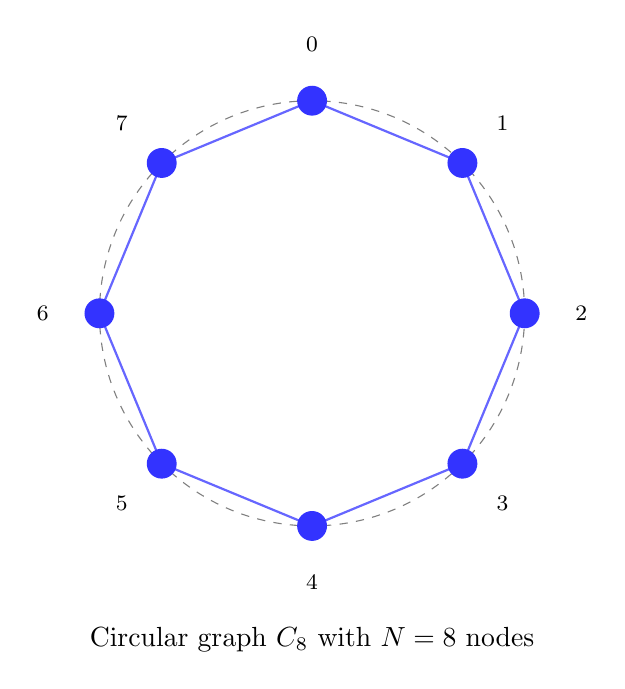
\begin{tikzpicture}[scale=1.8]
    \draw[gray, dashed] (0,0) circle (1.5);

    \foreach \i in {0,...,7} {
        \coordinate (n\i) at ({90 - \i*45}:1.5);
    }

    \draw[thick, blue!60] (n0) -- (n1);
    \draw[thick, blue!60] (n1) -- (n2);
    \draw[thick, blue!60] (n2) -- (n3);
    \draw[thick, blue!60] (n3) -- (n4);
    \draw[thick, blue!60] (n4) -- (n5);
    \draw[thick, blue!60] (n5) -- (n6);
    \draw[thick, blue!60] (n6) -- (n7);
    \draw[thick, blue!60] (n7) -- (n0);

    \foreach \i in {0,...,7} {
        \fill[blue!80] (n\i) circle (3pt);
        \node at ({90 - \i*45}:1.9) {\footnotesize $\i$};
    }

    \node at (0,-2.3) {Circular graph $C_8$ with $N = 8$ nodes};
\end{tikzpicture}
\caption{The circular graph. This structure has \emph{perfect
         translational symmetry}: every node ``looks the same'' as
         every other.}
\label{dft-to-gnn:fig:circular-graph}
\end{figure}

The adjacency matrix of $C_N$ is:
\begin{equation}
A_N = \begin{pmatrix}
0 & 1 & 0 & \cdots & 0 & 1 \\
1 & 0 & 1 & \cdots & 0 & 0 \\
0 & 1 & 0 & \cdots & 0 & 0 \\
\vdots & \vdots & \vdots & \ddots & \vdots & \vdots \\
0 & 0 & 0 & \cdots & 0 & 1 \\
1 & 0 & 0 & \cdots & 1 & 0
\end{pmatrix}
\end{equation}

Since every node has degree 2, the Laplacian is:
\begin{equation}
L_N = 2I - A_N
\end{equation}

\subsection{Finding the eigenvectors: the key calculation}

We seek signals $\mathbf{v}$ such that $L\mathbf{v} = \lambda\mathbf{v}$.
The Laplacian acts on component $j$ as:
\begin{equation}
(L\mathbf{v})_j = 2v_j - v_{j-1} - v_{j+1} = \lambda v_j
\end{equation}
which rearranges to:
\begin{equation}
v_{j-1} + v_{j+1} = (2 - \lambda) v_j
\label{dft-to-gnn:eq:recurrence}
\end{equation}

This is a \emph{linear recurrence relation}. Let us guess a solution
of the form:
\begin{equation}
v_j = e^{i\theta j}
\end{equation}
for some angle $\theta$. Substituting into \eqref{dft-to-gnn:eq:recurrence}:
\begin{align}
e^{i\theta(j-1)} + e^{i\theta(j+1)} &= (2 - \lambda) e^{i\theta j} \\
e^{-i\theta} + e^{i\theta} &= 2 - \lambda \\
2\cos\theta &= 2 - \lambda
\end{align}

So $\lambda = 2 - 2\cos\theta = 2(1 - \cos\theta)$.

But we also need \emph{periodicity}: the signal must satisfy
$v_N = v_0$ (we go around the whole circle and return). This requires:
\begin{equation}
e^{i\theta N} = e^{i\theta \cdot 0} = 1
\end{equation}
which means $\theta N = 2\pi k$ for some integer $k$, i.e.\
$\theta = \frac{2\pi k}{N}$.

\begin{theorem}[Eigenvectors of the circular graph Laplacian]
\label{dft-to-gnn:thm:circular-eigenvectors}
The eigenvectors of $L_N = 2I - A_N$ are:
\begin{equation}
\mathbf{v}_k = \frac{1}{\sqrt{N}}
\begin{pmatrix}
1 \\ e^{2\pi i k/N} \\ e^{2\pi i \cdot 2k/N} \\ \vdots \\
e^{2\pi i (N-1)k/N}
\end{pmatrix}, \quad k = 0, 1, \ldots, N-1
\end{equation}
with corresponding eigenvalues:
\begin{equation}
\lambda_k = 2 - 2\cos\left(\frac{2\pi k}{N}\right)
          = 4\sin^2\left(\frac{\pi k}{N}\right)
\end{equation}
These eigenvectors are orthonormal:
$\mathbf{v}_j^* \mathbf{v}_k = \delta_{jk}$.
\end{theorem}

\begin{figure}[H]
\centering
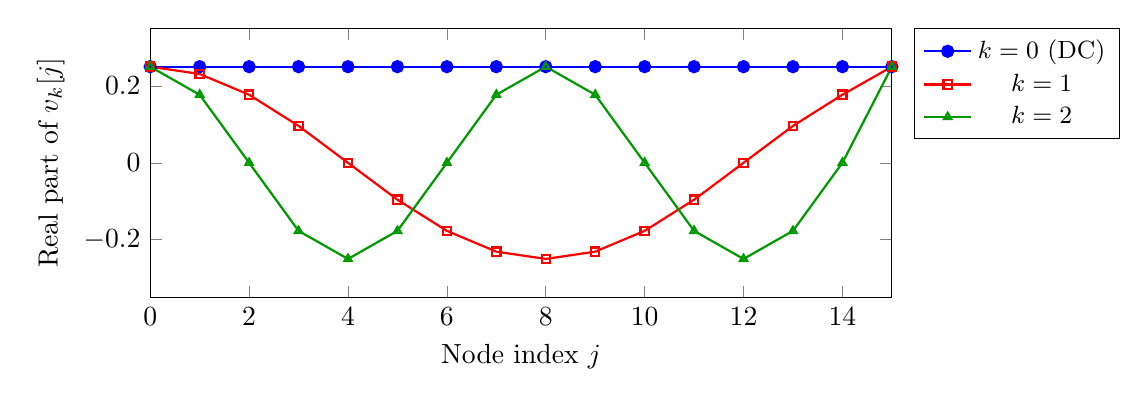
\begin{tikzpicture}
\begin{axis}[
    width=11cm, height=5cm, % Reduced width to create space for the legend
    xlabel={Node index $j$},
    ylabel={Real part of $v_k[j]$},
    xmin=0, xmax=15,
    ymin=-0.35, ymax=0.35,
    % Moves the legend outside the plotting area to the right
    legend pos=outer north east,
    legend style={font=\small},
]
% k=0 (constant)
\addplot[thick, blue, mark=*] coordinates {
    (0,0.25) (1,0.25) (2,0.25) (3,0.25) (4,0.25) (5,0.25) (6,0.25)
    (7,0.25) (8,0.25) (9,0.25) (10,0.25) (11,0.25) (12,0.25)
    (13,0.25) (14,0.25) (15,0.25)
};
\addlegendentry{$k=0$ (DC)}

% k=1
\addplot[thick, red, mark=square, mark size=1.5pt] coordinates {
    (0,0.25) (1,0.231) (2,0.177) (3,0.096) (4,0) (5,-0.096)
    (6,-0.177) (7,-0.231) (8,-0.25) (9,-0.231) (10,-0.177)
    (11,-0.096) (12,0) (13,0.096) (14,0.177) (15,0.25)
};
\addlegendentry{$k=1$}

% k=2
\addplot[thick, green!60!black, mark=triangle, mark size=1.5pt]
    coordinates {
    (0,0.25) (1,0.177) (2,0) (3,-0.177) (4,-0.25) (5,-0.177)
    (6,0) (7,0.177) (8,0.25) (9,0.177) (10,0) (11,-0.177)
    (12,-0.25) (13,-0.177) (14,0) (15,0.25)
};
\addlegendentry{$k=2$}
\end{axis}
\end{tikzpicture}

\caption{Real parts of the first three eigenvectors for $N=16$. These
         are samples of cosine waves at frequencies $0, 1, 2$ cycles
         around the circle.}
\label{dft-to-gnn:fig:cycle-eigvecs}
\end{figure}

\subsection{Interpretation: vibration modes}

Think of the circular graph as a ring of masses connected by springs.
The eigenvectors represent the natural \emph{vibration modes}:

\begin{itemize}
\item $k = 0$: All masses move together (rigid translation).
      Eigenvalue $\lambda_0 = 0$.
\item $k = 1$: One complete wave around the ring. Low eigenvalue
      (slow oscillation).
\item $k = N/2$ (if $N$ even): Alternating pattern $+,-,+,-,\ldots$.
      Highest eigenvalue (fastest oscillation).
\end{itemize}
Since $\lambda_k = \lambda_{N-k}$, every eigenvalue other than $\lambda_0$ (and $\lambda_{N/2}$ for even $N$) has multiplicity two: $\mathbf{v}_k$ and $\mathbf{v}_{N-k} = \overline{\mathbf{v}_k}$ span a plane that also contains the real vectors $\cos(2\pi kj/N)$ and $\sin(2\pi kj/N)$ (\cref{graph-laplacians:exr:4}). The eigenvalue fixes the frequency $\abs{k}$ but not the direction of travel around the ring.

\subsection{These are the DFT basis vectors}

Recall the DFT (\cref{fourier-analysis:def:dft}):
\begin{equation}
X_k = \sum_{n=0}^{N-1} x_n \, e^{-2\pi i kn/N}
\end{equation}

The $k$-th DFT coefficient is the inner product of the signal
$\mathbf{x}$ with the vector $\mathbf w_k$ of entries $e^{2\pi i kn/N}$, $n = 0, \ldots, N-1$, that is
\[
X_k = \mathbf w_k^*\mathbf x = \sqrt N\,\mathbf{v}_k^*\mathbf{x},
\]
where $\mathbf{v}_k^*$ is the conjugate transpose of our eigenvector $\mathbf{v}_k$.

\begin{keyidea}
The DFT basis vectors are the eigenvectors of
the circular graph Laplacian. The DFT is not an arbitrary choice: it
is forced by the circular symmetry of equally spaced points (\cref{dft-to-gnn:thm:app-forced-eigenfunctions}).
\end{keyidea}

\begin{remark}
Why are complex exponentials the eigenvectors? This is not a
coincidence --- it is a deep consequence of \emph{translation
invariance}. Any operator that commutes with circular shifts must
have complex exponentials as eigenfunctions. See
\cref{dft-to-gnn:app:translation-invariance} for a detailed proof.
\end{remark}

%==========================================================================
\section{The DFT as eigendecomposition}
%==========================================================================

\subsection{Matrix formulation}

As in \cref{ch:fourier-analysis}, the \emph{DFT matrix} $F \in \C^{N \times N}$ has entries
\begin{equation}
F_{kn} = e^{-2\pi i kn/N} = \omega^{kn},
\quad \text{where } \omega = e^{-2\pi i/N}
\end{equation}

so that $\mathbf{X} = F\mathbf{x}$ and $F^{-1} = \frac1N F^*$. (In this chapter $\omega$ denotes this root of unity; \cref{ch:fourier-analysis} called it $W_N$.)

\begin{example}[DFT matrix for $N = 4$]
With $\omega = e^{-2\pi i/4} = -i$:
\[
F_4 = \begin{pmatrix}
1 & 1 & 1 & 1 \\
1 & -i & -1 & i \\
1 & -1 & 1 & -1 \\
1 & i & -1 & -i
\end{pmatrix}
\]
The columns of $F^*$ (conjugate transpose) are the eigenvectors we
found: $(1, 1, 1, 1)$, $(1, i, -1, -i)$, $(1, -1, 1, -1)$,
$(1, -i, -1, i)$.
\end{example}

\subsection{The DFT diagonalizes the circular Laplacian}

\begin{theorem}[Diagonalization]
The circular graph Laplacian is diagonalized by the (normalized) DFT
matrix:
\begin{equation}
L_N = Q \Lambda Q^*
\end{equation}
where $Q = \frac{1}{\sqrt{N}} F^*$ has the eigenvectors as columns,
and $\Lambda = \diag(\lambda_0, \lambda_1, \ldots, \lambda_{N-1})$.
\end{theorem}

This means expressing a signal in the DFT basis is equivalent to
expressing it in the eigenbasis of the Laplacian. The DFT coefficient
$X_k$ measures how much of the $k$-th eigenvector (the $k$-th
``frequency mode'') is present in the signal.

\subsection{Frequency interpretation of eigenvalues}

The eigenvalues $\lambda_k = 4\sin^2(\pi k/N)$ have a natural
interpretation:

\begin{itemize}
\item $\lambda_0 = 0$: The constant signal. No variation between
      neighbours.
\item $\lambda_k$ small: Low-frequency modes. Slow variation around
      the circle.
\item $\lambda_k$ large: High-frequency modes. Rapid variation between
      neighbours.
\item $\lambda_{N/2} = 4$ (for even $N$): The alternating signal
      $(-1)^n$. Maximum variation.
\end{itemize}

\begin{figure}[H]
\centering
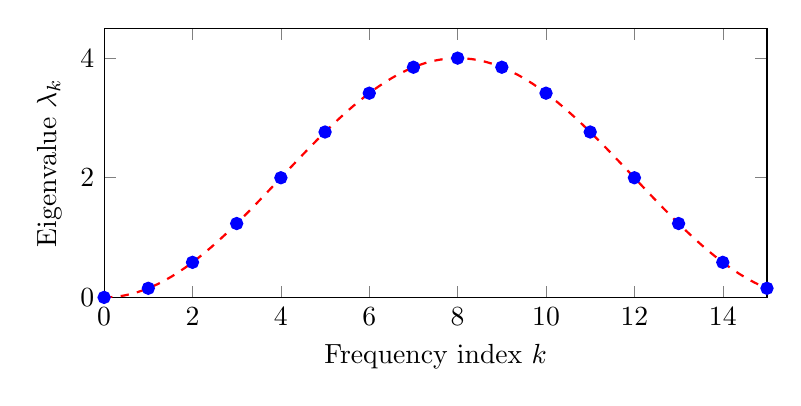
\begin{tikzpicture}
\begin{axis}[
    width=10cm, height=5cm,
    xlabel={Frequency index $k$},
    ylabel={Eigenvalue $\lambda_k$},
    xmin=0, xmax=15,
    ymin=0, ymax=4.5,
]
\addplot[thick, blue, mark=*, only marks] coordinates {
    (0, 0) (1, 0.152) (2, 0.586) (3, 1.235) (4, 2) (5, 2.765)
    (6, 3.414) (7, 3.848) (8, 4) (9, 3.848) (10, 3.414) (11, 2.765)
    (12, 2) (13, 1.235) (14, 0.586) (15, 0.152)
};
\addplot[thick, red, dashed, samples=100, domain=0:15]
    {4*sin(deg(pi*x/16))^2};
\end{axis}
\end{tikzpicture}
\caption{Eigenvalues $\lambda_k = 4\sin^2(\pi k/N)$ for $N=16$. Higher
         $k$ means higher eigenvalue (more variation).}
\end{figure}

%==========================================================================
\section{Convolution and the convolution theorem}
%==========================================================================

\subsection{Linear and circular convolution}

We use the two convolutions of \cref{ch:fourier-analysis}. For finite signals $x$ of length $N$ and $h$ of length $M$ (zero outside their supports), the \emph{linear} convolution $(x*h)[n] = \sum_m x[m]h[n-m]$ has length $N+M-1$. For two signals of the same length $N$, the \emph{circular} convolution (\cref{fourier-analysis:def:circular-convolution}) is $(x\circledast h)[n] = \sum_{m=0}^{N-1} x[m]\,h[(n-m)\bmod N]$; it has length $N$, and indices that fall off the end wrap around.

\begin{example}[Linear vs.\ circular convolution]
Let $x = [1, 2, 3]$ and $h = [1, 1]$.
\begin{itemize}
\item \textbf{Linear convolution}:
  \[
  y = x * h = [1\cdot1, 1\cdot1+2\cdot1, 2\cdot1+3\cdot1, 3\cdot1]
    = [1, 3, 5, 3]
  \]
  (length $3+2-1 = 4$).
\item \textbf{Circular convolution} (pad $h$ to length 3: $[1, 1, 0]$):
  \begin{align*}
  y[0] &= x[0]h[0] + x[1]h[2] + x[2]h[1] = 1\cdot1 + 2\cdot0 + 3\cdot1 = 4 \\
  y[1] &= x[0]h[1] + x[1]h[0] + x[2]h[2] = 1\cdot1 + 2\cdot1 + 3\cdot0 = 3 \\
  y[2] &= x[0]h[2] + x[1]h[1] + x[2]h[0] = 1\cdot0 + 2\cdot1 + 3\cdot1 = 5
  \end{align*}
  So $y = x \circledast h = [4, 3, 5]$ (length 3).
\end{itemize}
The circular convolution has a different first entry ($4$ instead of $1$) because of wrap-around: the term $x[2]h[(0-2)\bmod 3] = x[2]h[1] = 3$ is the last entry $y[3] = 3$ of the linear convolution, folded back onto index $0$. In general the circular convolution of length $N$ is the linear convolution with entries $n$ and $n+N$ added together.
\end{example}

\subsection{Circulant matrices represent circular convolution}

Circular convolution can be written as a matrix-vector product
$\mathbf{y} = C_h \mathbf{x}$, where $C_h$ is a \emph{circulant
matrix}:

\begin{equation}
C_h = \begin{pmatrix}
h_0 & h_{N-1} & h_{N-2} & \cdots & h_1 \\
h_1 & h_0 & h_{N-1} & \cdots & h_2 \\
h_2 & h_1 & h_0 & \cdots & h_3 \\
\vdots & \vdots & \vdots & \ddots & \vdots \\
h_{N-1} & h_{N-2} & h_{N-3} & \cdots & h_0
\end{pmatrix}
\end{equation}

Each row is a cyclic shift of the previous one. The $(i,j)$ entry is
$C_{ij} = h_{(i-j) \bmod N}$.

\subsection{Circulant matrices and the DFT}

\begin{theorem}[All circulant matrices share the same eigenvectors]
\label{dft-to-gnn:thm:circulant-eigenvectors}
Every circulant matrix $C$ is diagonalized by the DFT matrix:
\begin{equation}
C = F^{-1} \, \diag(\text{DFT}(\mathbf{c})) \, F
\end{equation}
where $\mathbf{c} = (c_0, c_1, \ldots, c_{N-1})^\top$ is the first column
of $C$.
\end{theorem}

\begin{proof}[Detailed proof]
Let $C$ be a circulant matrix with first column $\mathbf{c} =
(c_0, c_1, \ldots, c_{N-1})^\top$. The $(i,j)$ entry is:
\[
C_{ij} = c_{(i-j) \bmod N}
\]

Let $\mathbf{v}_k$ be the $k$-th DFT basis vector (normalized):
\[
\mathbf{v}_k = \frac{1}{\sqrt{N}}
\begin{pmatrix}
1 \\ e^{2\pi i k/N} \\ e^{4\pi i k/N} \\ \vdots \\ e^{2\pi i (N-1)k/N}
\end{pmatrix}
\]

Compute $(C\mathbf{v}_k)[n]$:
\begin{align*}
(C\mathbf{v}_k)[n]
    &= \sum_{m=0}^{N-1} C_{nm} \mathbf{v}_k[m] \\
    &= \sum_{m=0}^{N-1} c_{(n-m) \bmod N} \cdot \frac{1}{\sqrt{N}}
       e^{2\pi i mk/N}
\end{align*}

Change variable: $\ell = (n-m) \bmod N$, so $m = (n-\ell) \bmod N$, and
$e^{2\pi i mk/N} = e^{2\pi i (n-\ell)k/N} = e^{2\pi i nk/N}
\cdot e^{-2\pi i \ell k/N}$:

\begin{align*}
(C\mathbf{v}_k)[n]
    &= \frac{1}{\sqrt{N}} \sum_{\ell=0}^{N-1} c_\ell
       \left( e^{2\pi i nk/N} \cdot e^{-2\pi i \ell k/N} \right) \\
    &= \frac{1}{\sqrt{N}} e^{2\pi i nk/N}
       \sum_{\ell=0}^{N-1} c_\ell \, e^{-2\pi i \ell k/N} \\
    &= \mathbf{v}_k[n] \cdot \underbrace{\sum_{\ell=0}^{N-1} c_\ell
       e^{-2\pi i \ell k/N}}_{\text{DFT}(\mathbf{c})_k}
\end{align*}

Thus $C\mathbf{v}_k = \text{DFT}(\mathbf{c})_k \cdot \mathbf{v}_k$,
proving $\mathbf{v}_k$ is an eigenvector with eigenvalue
$\text{DFT}(\mathbf{c})_k$. This holds for all circulant matrices $C$
using the same eigenvectors $\mathbf{v}_k$.
\end{proof}

\paragraph{Key insight.} The circular graph Laplacian $L_N = 2I - A_N$ is
itself a circulant matrix. \Cref{dft-to-gnn:thm:circulant-eigenvectors}
tells us that \emph{all} circulant matrices --- including all
\emph{circular convolution} operators --- share the same eigenvectors:
the DFT basis.

\subsection{The convolution theorem for circular convolution}

\begin{theorem}[Convolution theorem for circular convolution]
\label{dft-to-gnn:thm:convolution-circular}
Let $\mathbf{X} = \text{DFT}(\mathbf{x})$,
$\mathbf{H} = \text{DFT}(\mathbf{h})$, and
$\mathbf{Y} = \text{DFT}(\mathbf{x} \circledast \mathbf{h})$, where
$\circledast$ denotes \emph{circular convolution}. Then:
\begin{equation}
Y_k = X_k \cdot H_k \quad \text{for all } k
\end{equation}
\emph{Circular convolution in the time domain equals pointwise
multiplication in the frequency domain.}
\end{theorem}

\begin{proof}
Since circular convolution corresponds to multiplication by a circulant
matrix $\mathbf{y} = C_h \mathbf{x}$, and we just showed $C_h$ is
diagonalized by the DFT:
\begin{equation}
\mathbf{Y} = F\mathbf{y} = F C_h \mathbf{x}
           = F C_h F^{-1} \cdot F\mathbf{x}
           = \diag(\mathbf{H}) \cdot \mathbf{X}
\end{equation}
which is componentwise multiplication.
\end{proof}

\subsection{Linear convolution via DFT with zero padding}

The DFT naturally gives us \emph{circular convolution}, but we often
want \emph{linear convolution}. The solution is \emph{zero padding}:

\begin{theorem}[Linear convolution via DFT]
Given $x[n]$ (length $N$) and $h[n]$ (length $M$), let $L \geq N+M-1$.
Define zero-padded versions:
\begin{align*}
x_{\text{pad}}[n] &= \begin{cases}
x[n] & 0 \leq n < N \\
0 & N \leq n < L
\end{cases} \\
h_{\text{pad}}[n] &= \begin{cases}
h[n] & 0 \leq n < M \\
0 & M \leq n < L
\end{cases}
\end{align*}
Then the linear convolution $y = x * h$ can be computed as:
\begin{equation}
y[n] = \text{IDFT}\left(\text{DFT}(x_{\text{pad}}) \odot
       \text{DFT}(h_{\text{pad}})\right)[n]
\end{equation}
for $0 \leq n \leq N+M-2$, where $\odot$ denotes elementwise
multiplication.
\end{theorem}

\begin{proof}
By the circular convolution theorem (\cref{dft-to-gnn:thm:convolution-circular}) the right side is $(x_{\text{pad}}\circledast h_{\text{pad}})[n] = \sum_{m=0}^{L-1} x_{\text{pad}}[m]\,h_{\text{pad}}[(n-m)\bmod L]$. Only $0\le m\le N-1$ contribute. For such $m$ and $0\le n\le N+M-2$ we have $-(N-1) \le n-m \le N+M-2$. If $n - m \ge 0$ the index is $n-m$ itself (as $n-m \le N+M-2 < L$); if $n-m<0$ the index is $L+n-m \ge L-(N-1) \ge M$, where $h_{\text{pad}}$ vanishes. In both cases $h_{\text{pad}}[(n-m)\bmod L] = h[n-m]$ with the convention $h[k] = 0$ outside $0\le k\le M-1$, so the sum is $\sum_m x[m]h[n-m] = (x*h)[n]$.
\end{proof}

\subsection{Detailed example: computing linear convolution via DFT}

Let us work through a complete example to see exactly how zero-padding allows us to compute
linear convolution using the DFT.

\begin{example}[Computing linear convolution via the DFT, in detail]
Let $x = [1, 2, 3]$ ($N=3$) and $h = [1, 1]$ ($M=2$). The linear convolution should yield:
\[
y = x * h = [1, 3, 5, 3]
\]
with length $L_y = N + M - 1 = 3 + 2 - 1 = 4$.

Indeed, the convolution is defined by the formula:
\[
y[n] = \sum_{k=-\infty}^{\infty} x[k]h[n-k]
\]
Therefore:
\begin{align*}
    y[0] &= x[0]h[0] = 1 \cdot 1 = 1 \\
    y[1] &= x[0]h[1] + x[1]h[0] = (1 \cdot 1) + (2 \cdot 1) = 3 \\
    y[2] &= x[1]h[1] + x[2]h[0] = (2 \cdot 1) + (3 \cdot 1) = 5 \\
    y[3] &= x[2]h[1] = 3 \cdot 1 = 3
\end{align*}


\vspace{0.3cm}
\emph{Step 1: zero-padding.}
We need to pad both signals to length $L \geq N + M - 1 = 4$. Let us choose $L = 4$:
\begin{align*}
x_{\text{pad}} &= [1, 2, 3, 0] \\
h_{\text{pad}} &= [1, 1, 0, 0]
\end{align*}

\vspace{0.3cm}
\emph{Step 2: compute DFTs.}
For $L=4$, the DFT matrix uses $\omega = e^{-2\pi i/4} = e^{-\pi i/2} = -i$.

The DFT matrix is:
\[
F_4 = \begin{pmatrix}
1 & 1 & 1 & 1 \\
1 & -i & -1 & i \\
1 & -1 & 1 & -1 \\
1 & i & -1 & -i
\end{pmatrix}
\]

Compute $\mathbf{X} = F_4 x_{\text{pad}}$:
\begin{align*}
X[0] &= 1 + 2 + 3 + 0 = 6 \\
X[1] &= 1 + 2(-i) + 3(-1) + 0(i) = 1 - 2i - 3 = -2 - 2i \\
X[2] &= 1 + 2(-1) + 3(1) + 0(-1) = 1 - 2 + 3 = 2 \\
X[3] &= 1 + 2(i) + 3(-1) + 0(-i) = 1 + 2i - 3 = -2 + 2i
\end{align*}
So $\mathbf{X} = [6, -2-2i, 2, -2+2i]$.

Compute $\mathbf{H} = F_4 h_{\text{pad}}$:
\begin{align*}
H[0] &= 1 + 1 + 0 + 0 = 2 \\
H[1] &= 1 + 1(-i) + 0(-1) + 0(i) = 1 - i \\
H[2] &= 1 + 1(-1) + 0(1) + 0(-1) = 1 - 1 = 0 \\
H[3] &= 1 + 1(i) + 0(-1) + 0(-i) = 1 + i
\end{align*}
So $\mathbf{H} = [2, 1-i, 0, 1+i]$.

\vspace{0.3cm}
\emph{Step 3: multiply in frequency domain.}
Elementwise multiplication: $Y[k] = X[k] \cdot H[k]$
\begin{align*}
Y[0] &= 6 \times 2 = 12 \\
Y[1] &= (-2-2i) \times (1-i) = (-2-2i)(1-i) = -2(1-i) -2i(1-i) \\
     &= -2 + 2i - 2i + 2i^2 = -2 - 2 = -4 \quad (\text{since } i^2 = -1) \\
Y[2] &= 2 \times 0 = 0 \\
Y[3] &= (-2+2i) \times (1+i) = (-2+2i)(1+i) = -2(1+i) + 2i(1+i) \\
     &= -2 - 2i + 2i + 2i^2 = -2 - 2 = -4
\end{align*}
So $\mathbf{Y} = [12, -4, 0, -4]$.

\vspace{0.3cm}
\emph{Step 4: inverse DFT.}
The inverse DFT matrix is $F_4^{-1} = \frac{1}{4} F_4^*$ (conjugate transpose).

Compute $\mathbf{y} = F_4^{-1} \mathbf{Y} = \frac{1}{4} F_4^* \mathbf{Y}$:
\[
F_4^* = \begin{pmatrix}
1 & 1 & 1 & 1 \\
1 & i & -1 & -i \\
1 & -1 & 1 & -1 \\
1 & -i & -1 & i
\end{pmatrix}
\]

\begin{align*}
y[0] &= \frac{1}{4}[1\cdot 12 + 1\cdot(-4) + 1\cdot 0 + 1\cdot(-4)] =
\frac{1}{4}(12 - 4 + 0 - 4) = \frac{4}{4} = 1 \\
y[1] &= \frac{1}{4}[1\cdot 12 + i\cdot(-4) + (-1)\cdot 0 + (-i)\cdot(-4)] \\
     &= \frac{1}{4}(12 - 4i + 0 + 4i) = \frac{12}{4} = 3 \\
y[2] &= \frac{1}{4}[1\cdot 12 + (-1)\cdot(-4) + 1\cdot 0 + (-1)\cdot(-4)] \\
     &= \frac{1}{4}(12 + 4 + 0 + 4) = \frac{20}{4} = 5 \\
y[3] &= \frac{1}{4}[1\cdot 12 + (-i)\cdot(-4) + (-1)\cdot 0 + i\cdot(-4)] \\
     &= \frac{1}{4}(12 + 4i + 0 - 4i) = \frac{12}{4} = 3
\end{align*}

So $\mathbf{y} = [1, 3, 5, 3]$, which matches the direct linear convolution.

\vspace{0.3cm}
\emph{Why this worked.} Without padding (length $3$) we found $y_{\text{circ}} = [4, 3, 5]$ in the previous example: the last entry of the linear convolution wrapped around onto index $0$. With length $L = 4 = N+M-1$ there is room for all four entries, and the wrapped-around terms involve $x_{\text{pad}}[3] = 0$ or $h_{\text{pad}}[2] = h_{\text{pad}}[3] = 0$, so they vanish. This is exactly the index argument in the proof above.

\end{example}

\subsection{Visualizing how zero-padding works}

\begin{figure}[H]
\centering
\resizebox{\linewidth}{!}{%
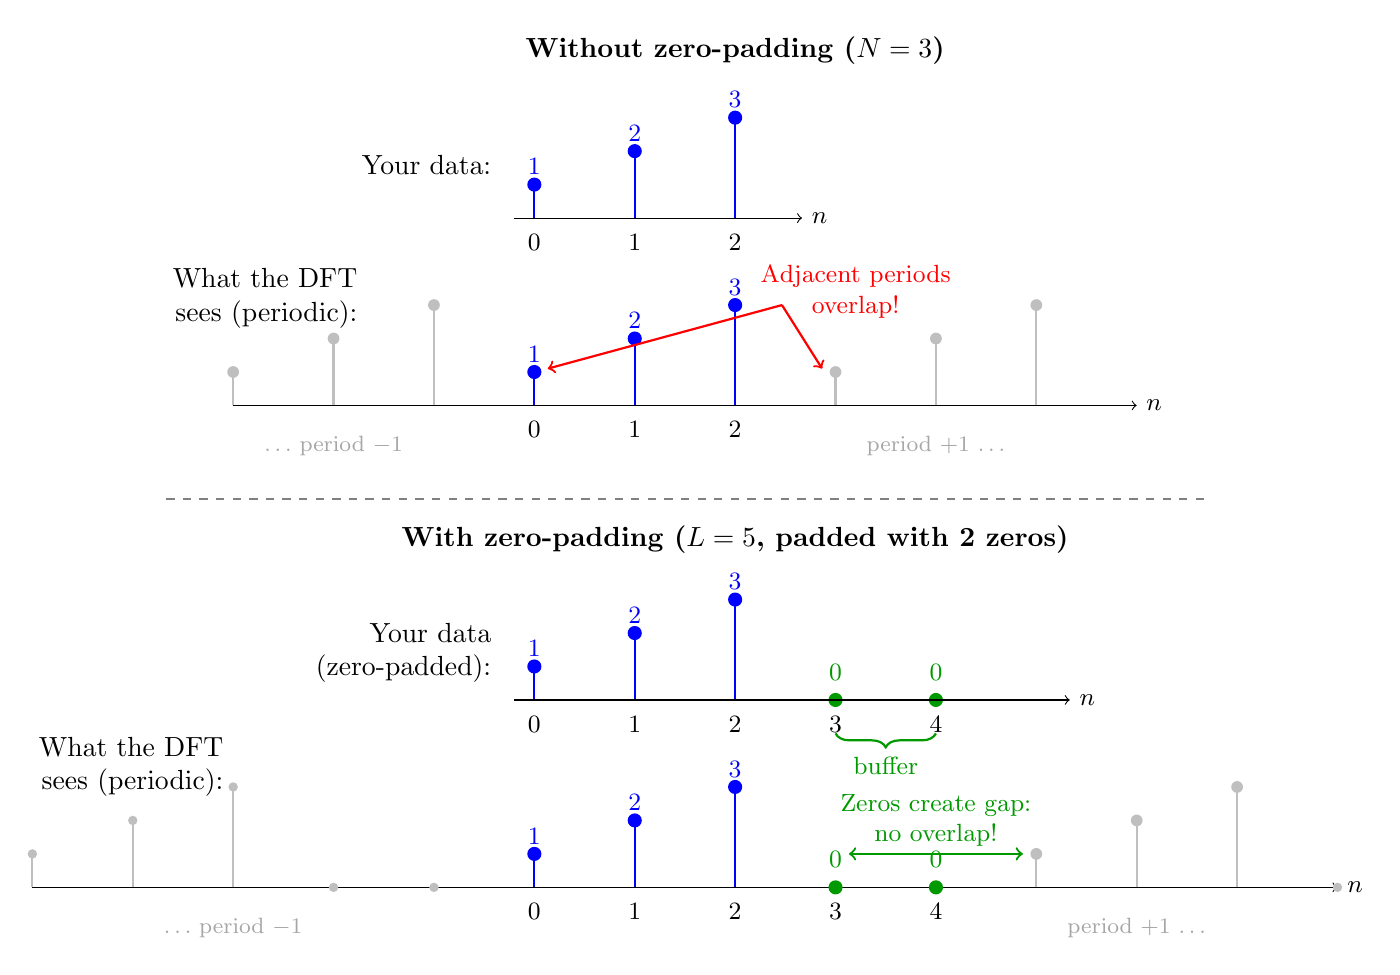
\begin{tikzpicture}[scale=0.85]

    % ===== WITHOUT ZERO-PADDING =====
    \node[font=\bfseries] at (3, 5.7) {Without zero-padding ($N=3$)};

    % Label for "Your data"
    \node[anchor=east] at (-0.5, 4) {Your data:};

    % Draw signal x as stem plot
    \foreach \n/\val in {0/1, 1/2, 2/3} {
        \draw[thick, blue] (\n*1.5, 3.2) -- (\n*1.5, 3.2 + \val*0.5);
        \fill[blue] (\n*1.5, 3.2 + \val*0.5) circle (3pt);
        \node[below, font=\small] at (\n*1.5, 3.1) {$\n$};
        \node[above, font=\small, blue] at (\n*1.5, 3.2 + \val*0.5) {\val};
    }
    \draw[->] (-0.3, 3.2) -- (4, 3.2) node[right, font=\small] {$n$};

    % Label for "What DFT sees"
    \node[anchor=east, align=right] at (-2.5, 2) {What the DFT\\sees (periodic):};

    % Draw periodic extension
    \draw[->] (-4.5, 0.4) -- (9, 0.4) node[right, font=\small] {$n$};

    % Previous period (gray)
    \foreach \n/\val in {0/1, 1/2, 2/3} {
        \pgfmathsetmacro{\xpos}{-4.5 + \n*1.5}
        \draw[thick, gray!50] (\xpos, 0.4) -- (\xpos, 0.4 + \val*0.5);
        \fill[gray!50] (\xpos, 0.4 + \val*0.5) circle (2.5pt);
    }
    \node[gray!70, font=\footnotesize] at (-3, -0.2) {$\ldots$ period $-1$};

    % Current period (blue) - indices 0,1,2
    \foreach \n/\val in {0/1, 1/2, 2/3} {
        \draw[thick, blue] (\n*1.5, 0.4) -- (\n*1.5, 0.4 + \val*0.5);
        \fill[blue] (\n*1.5, 0.4 + \val*0.5) circle (3pt);
        \node[below, font=\small] at (\n*1.5, 0.3) {$\n$};
        \node[above, font=\small, blue] at (\n*1.5, 0.4 + \val*0.5) {\val};
    }

    % Next period (gray) - shows wrap-around
    \foreach \n/\val in {0/1, 1/2, 2/3} {
        \pgfmathsetmacro{\xpos}{4.5 + \n*1.5}
        \draw[thick, gray!50] (\xpos, 0.4) -- (\xpos, 0.4 + \val*0.5);
        \fill[gray!50] (\xpos, 0.4 + \val*0.5) circle (2.5pt);
    }
    \node[gray!70, font=\footnotesize] at (6, -0.2) {period $+1$ $\ldots$};

    % Highlight wrap-around problem
    \draw[red, thick, ->] (3.7, 1.9) -- (4.3, 0.95);
    \draw[red, thick, ->] (3.7, 1.9) -- (0.2, 0.95);
    \node[red, font=\small, align=center] at (4.8, 2.1) {Adjacent periods\\overlap!};

    % Vertical separator
    \draw[thick, gray, dashed] (-5.5, -1) -- (10, -1);

    % ===== WITH ZERO-PADDING =====
    \node[font=\bfseries] at (3, -1.6) {With zero-padding ($L=5$, padded with 2 zeros)};

    % Label for "Your data (padded)"
    \node[anchor=east, align=right] at (-0.5, -3.3) {Your data\\(zero-padded):};

    % Draw zero-padded signal
    \foreach \n/\val in {0/1, 1/2, 2/3} {
        \draw[thick, blue] (\n*1.5, -4) -- (\n*1.5, -4 + \val*0.5);
        \fill[blue] (\n*1.5, -4 + \val*0.5) circle (3pt);
        \node[below, font=\small] at (\n*1.5, -4.1) {$\n$};
        \node[above, font=\small, blue] at (\n*1.5, -4 + \val*0.5) {\val};
    }
    % Zeros
    \foreach \n in {3, 4} {
        \draw[thick, green!60!black] (\n*1.5, -4) -- (\n*1.5, -4);
        \fill[green!60!black] (\n*1.5, -4) circle (3pt);
        \node[below, font=\small] at (\n*1.5, -4.1) {$\n$};
        \node[above, font=\small, green!60!black] at (\n*1.5, -3.85) {0};
    }
    \draw[->] (-0.3, -4) -- (8, -4) node[right, font=\small] {$n$};

    % Brace for zeros
    \draw[decorate, decoration={brace, amplitude=5pt, mirror},
          green!60!black, thick]
        (4.5, -4.5) -- (6, -4.5) node[midway, below=5pt,
                                      font=\small, green!60!black] {buffer};

    % Label for "What DFT sees"
    \node[anchor=east, align=right] at (-4.5, -5.0) {What the DFT\\sees (periodic):};

    % Draw periodic extension with zeros
    \draw[->] (-7.5, -6.8) -- (12, -6.8) node[right, font=\small] {$n$};

    % Previous period (gray) with zeros at end
    \foreach \n/\val in {0/1, 1/2, 2/3} {
        \pgfmathsetmacro{\xpos}{-7.5 + \n*1.5}
        \draw[thick, gray!50] (\xpos, -6.8) -- (\xpos, -6.8 + \val*0.5);
        \fill[gray!50] (\xpos, -6.8 + \val*0.5) circle (2pt);
    }
    \foreach \n in {3, 4} {
        \pgfmathsetmacro{\xpos}{-7.5 + \n*1.5}
        \fill[gray!50] (\xpos, -6.8) circle (2pt);
    }
    \node[gray!70, font=\footnotesize] at (-4.5, -7.4) {$\ldots$ period $-1$};

    % Current period (blue + green zeros)
    \foreach \n/\val in {0/1, 1/2, 2/3} {
        \draw[thick, blue] (\n*1.5, -6.8) -- (\n*1.5, -6.8 + \val*0.5);
        \fill[blue] (\n*1.5, -6.8 + \val*0.5) circle (3pt);
        \node[below, font=\small] at (\n*1.5, -6.9) {$\n$};
        \node[above, font=\small, blue] at (\n*1.5, -6.8 + \val*0.5) {\val};
    }
    \foreach \n in {3, 4} {
        \fill[green!60!black] (\n*1.5, -6.8) circle (3pt);
        \node[below, font=\small] at (\n*1.5, -6.9) {$\n$};
        \node[above, font=\small, green!60!black] at (\n*1.5, -6.65) {0};
    }

    % Next period (gray)
    \foreach \n/\val in {0/1, 1/2, 2/3} {
        \pgfmathsetmacro{\xpos}{7.5 + \n*1.5}
        \draw[thick, gray!50] (\xpos, -6.8) -- (\xpos, -6.8 + \val*0.5);
        \fill[gray!50] (\xpos, -6.8 + \val*0.5) circle (2.5pt);
    }
    \foreach \n in {3} {
        \pgfmathsetmacro{\xpos}{7.5 + \n*1.5}
        \fill[gray!50] (\xpos, -6.8) circle (2pt);
    }
    \node[gray!70, font=\footnotesize] at (9, -7.4) {period $+1$ $\ldots$};

    % Show the gap created by zeros
    \draw[green!60!black, thick, <->] (4.7, -6.3) -- (7.3, -6.3);
    \node[green!60!black, font=\small, align=center] at (6, -5.8)
        {Zeros create gap:\\no overlap!};

\end{tikzpicture}%
}
\caption{Zero-padding prevents wrap-around interference. Top:
         Without padding, the DFT treats the signal as periodic, so
         adjacent copies overlap during circular convolution.
         Bottom: With zero-padding, the zeros create a buffer
         zone between periods, preventing interference.}
\end{figure}

\paragraph{Key insight.} When we zero-pad to length $L \geq N+M-1$, the circular convolution
of the padded signals has no ``wrap-around interference'' in the first $N+M-1$ samples.
The zeros act as a buffer that isolates one period from the next in the DFT's implicit
periodic extension.

\begin{remark}[DFT periodicity and zero padding]
The DFT formula applies to any finite sequence, but it treats the sequence as one period of an $N$-periodic signal $x[n\bmod N]$. Zero padding to length $L$ changes the period to $L$; the appended zeros separate consecutive copies of the signal, so that a filter of length $M$ never reaches from one copy into the next.
\end{remark}

\subsection{Computational efficiency: why this matters}

Direct linear convolution takes $O(NM)$ operations. Using the FFT with
zero-padding:

\begin{enumerate}
\item Zero-pad to $L \approx N+M$: $O(L)$.
\item Compute $\mathbf{X} = \text{FFT}(\mathbf{x}_{\text{pad}})$: $O(L \log L)$.
\item Compute $\mathbf{H} = \text{FFT}(\mathbf{h}_{\text{pad}})$: $O(L \log L)$.
\item Multiply: $Y_k = X_k \cdot H_k$: $O(L)$.
\item Compute $\mathbf{y} = \text{IFFT}(\mathbf{Y})$: $O(L \log L)$.
\end{enumerate}

Total: $O(L \log L)$ instead of $O(NM)$. For large $N, M$, this is a
dramatic speedup.

\begin{example}[Speedup comparison]
For $N = M = 10^6$:
\begin{itemize}
\item Direct convolution: $\sim 10^{12}$ operations.
\item FFT-based convolution (with $L \approx 2\times10^6$):
      $\sim 2\times10^6 \times \log_2(2\times10^6) \approx 4\times10^7$
      operations.
\item Ratio: about $2.5\times10^4$; counting the three transforms and the constant of the FFT (\cref{ch:fourier-analysis}) lowers this by a small factor, so the gain is still about four orders of magnitude.
\end{itemize}
\end{example}

%==========================================================================
\section{Generalization: the graph Fourier transform}
%==========================================================================

We have seen that the DFT is the \emph{natural} frequency analysis for the
circular graph. What about arbitrary graphs? This question leads to
\emph{spectral graph theory} (Chung, \emph{Spectral Graph Theory}, 1997) and to signal processing on graphs (Shuman et al., \emph{The Emerging Field of Signal Processing on Graphs}, 2013).

\subsection{The key idea}

The essential insight from the circular case is:

\begin{keyidea}
The eigenvectors of the graph Laplacian define a \emph{frequency basis} for signals on that graph.
\end{keyidea}

For the circular graph, these eigenvectors happen to be complex
exponentials (the DFT basis) because of the special symmetry. For
general graphs, the eigenvectors are more complicated, but the
principle is the same.

\subsection{Definition of the graph Fourier transform}

We recall the graph Fourier transform of \cref{graph-laplacians:def:gft}, in matrix form and with eigenvalues in increasing order.

\begin{definition}[Graph Fourier transform]\label{dft-to-gnn:def:gft}
Let $G$ be an undirected graph with Laplacian $L$ having eigendecomposition:
\begin{equation}
L = U \Lambda U^\top
\end{equation}
where $U = [\mathbf{u}_0 | \mathbf{u}_1 | \cdots | \mathbf{u}_{N-1}]$
has orthonormal eigenvectors as columns, and
$\Lambda = \diag(\lambda_0, \ldots, \lambda_{N-1})$ with
$0 = \lambda_0 \leq \lambda_1 \leq \cdots \leq \lambda_{N-1}$.

The \emph{Graph Fourier Transform (GFT)} of signal $\mathbf{x}$ is:
\begin{equation}
\hat{\mathbf{x}} = U^\top \mathbf{x}
\end{equation}
The \emph{inverse GFT} is:
\begin{equation}
\mathbf{x} = U \hat{\mathbf{x}}
\end{equation}
\end{definition}

\begin{remark}
The coefficient $\hat{x}_k = \mathbf{u}_k^\top \mathbf{x}$ measures how
much of the $k$-th eigenvector is present in $\mathbf{x}$. Eigenvectors
with low $\lambda_k$ are ``smooth'' (low variation); those with high
$\lambda_k$ are ``rough'' (high variation). The GFT decomposes a signal
into components of increasing ``frequency'' on the graph.
\end{remark}

\subsection{Example: path graph}

Consider a path graph with 4 nodes:

\begin{figure}[H]
\centering
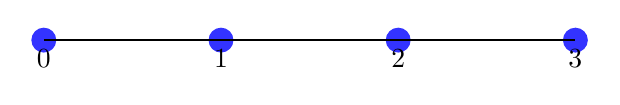
\begin{tikzpicture}[scale=1.5]
    \foreach \i in {0,...,3} {
        \coordinate (n\i) at (\i*1.5, 0);
        \fill[blue!80] (n\i) circle (3pt);
        \node[below] at (n\i) {$\i$};
    }
    \draw[thick] (n0) -- (n1) -- (n2) -- (n3);
\end{tikzpicture}
\caption{Path graph $P_4$.}
\end{figure}

The Laplacian is:
\begin{equation}
L = \begin{pmatrix}
1 & -1 & 0 & 0 \\
-1 & 2 & -1 & 0 \\
0 & -1 & 2 & -1 \\
0 & 0 & -1 & 1
\end{pmatrix}
\end{equation}

The eigenvalues and eigenvectors (exactly) are:

\begin{align*}
\lambda_0 &= 0, \quad \mathbf{u}_0 = \frac{1}{2}(1, 1, 1, 1)^\top \\
\lambda_1 &= 2 - \sqrt{2} \approx 0.586, \quad
           \mathbf{u}_1 \propto (1, \sqrt{2}-1, 1-\sqrt{2}, -1)^\top, \\ &\qquad\text{normalized: } \mathbf{u}_1 \approx (0.653, 0.271, -0.271, -0.653)^\top \\
\lambda_2 &= 2, \quad \mathbf{u}_2 = \frac{1}{2}(1, -1, -1, 1)^\top \\
\lambda_3 &= 2 + \sqrt{2} \approx 3.414, \quad
           \mathbf{u}_3 \propto (1, -\sqrt{2}-1, \sqrt{2}+1, -1)^\top, \\ &\qquad\text{normalized: } \mathbf{u}_3 \approx (0.271, -0.653, 0.653, -0.271)^\top
\end{align*}

\begin{figure}[H]
\centering
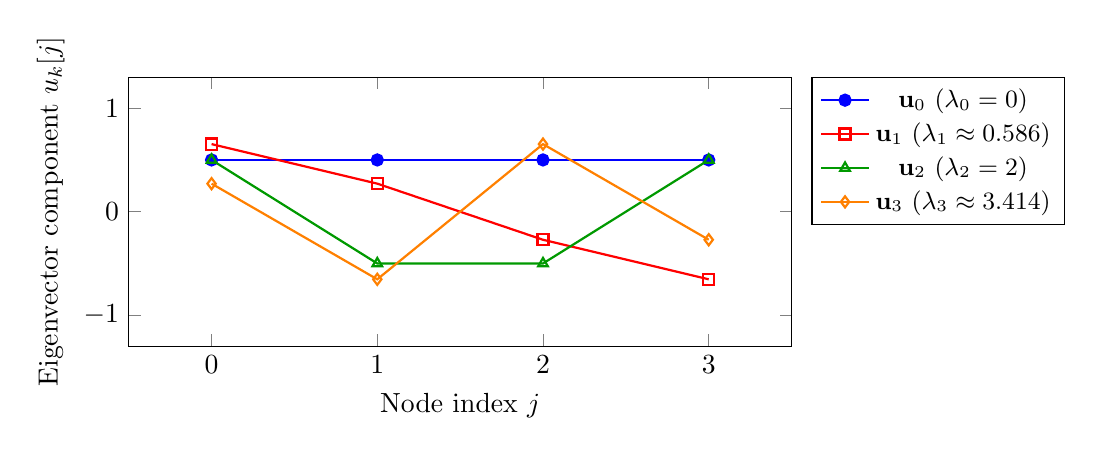
\begin{tikzpicture}
\begin{axis}[
    width=10cm, height=5cm,
    xlabel={Node index $j$},
    ylabel={Eigenvector component $u_k[j]$},
    xmin=-0.5, xmax=3.5,
    ymin=-1.3, ymax=1.3,
    legend pos=outer north east,
    legend style={font=\small},
    xtick={0,1,2,3},
]
% u0
\addplot[thick, blue, mark=*] coordinates {
    (0,0.5) (1,0.5) (2,0.5) (3,0.5)
};
\addlegendentry{$\mathbf{u}_0$ ($\lambda_0=0$)}

% u1
\addplot[thick, red, mark=square] coordinates {
    (0,0.653) (1,0.271) (2,-0.271) (3,-0.653)
};
\addlegendentry{$\mathbf{u}_1$ ($\lambda_1\approx0.586$)}

% u2
\addplot[thick, green!60!black, mark=triangle] coordinates {
    (0,0.5) (1,-0.5) (2,-0.5) (3,0.5)
};
\addlegendentry{$\mathbf{u}_2$ ($\lambda_2=2$)}

% u3
\addplot[thick, orange, mark=diamond] coordinates {
    (0,0.271) (1,-0.653) (2,0.653) (3,-0.271)
};
\addlegendentry{$\mathbf{u}_3$ ($\lambda_3\approx3.414$)}
\end{axis}
\end{tikzpicture}
\caption{Eigenvectors of the path graph $P_4$. These look like discretized
         cosines, similar to DFT basis vectors but adapted to the path's
         boundary conditions.}
\end{figure}

These eigenvectors look like discretized cosines --- similar to the DFT,
but adapted to the boundary conditions of the path. This is not a
coincidence: the path graph eigenvectors are exactly the Discrete
Cosine Transform (DCT) basis (\cref{dft-to-gnn:app:dct-path}). The eigenvector $\mathbf{u}_k$ changes sign exactly $k$ times along the path: $\mathbf{u}_0$ is constant, $\mathbf{u}_1$ goes from positive to negative once, and $\mathbf{u}_3$ alternates in sign at every edge. The number of sign changes grows with the eigenvalue, just as the number of oscillations grows with the frequency $k$ of a DFT basis vector.

%==========================================================================
\section{Spectral graph convolution}
%==========================================================================

\subsection{The problem: what is convolution on a graph?}

On regular structures (like the circle or grid), convolution slides a
filter across the signal. But on an irregular graph, there is no
consistent notion of ``sliding'' --- the neighbourhood structure varies
from node to node.

However, we can define convolution \emph{spectrally}:

\begin{keyidea}
Since convolution becomes multiplication
in the frequency domain, we \emph{define} graph convolution as
multiplication in the Graph Fourier domain.
\end{keyidea}

\subsection{Definition of spectral graph convolution}

\begin{definition}[Spectral graph convolution]
The spectral convolution of signal $\mathbf{x}$ with filter $g$ on
graph $G$ is:
\begin{equation}
\mathbf{x} *_G g = U \, g(\Lambda) \, U^\top \mathbf{x}
\end{equation}
where $g(\Lambda) = \diag(g(\lambda_0), g(\lambda_1), \ldots,
g(\lambda_{N-1}))$ is the filter applied to each eigenvalue.
\end{definition}

In other words:
\begin{enumerate}
\item Transform to the graph spectral domain:
      $\hat{\mathbf{x}} = U^\top \mathbf{x}$.
\item Multiply by the filter's frequency response:
      $\hat{\mathbf{y}}_k = g(\lambda_k) \cdot \hat{\mathbf{x}}_k$.
\item Transform back: $\mathbf{y} = U \hat{\mathbf{y}}$.
\end{enumerate}

\subsection{Low-pass, high-pass and band-pass filters}

The filter function $g$ decides which graph frequencies are kept. Because small $\lambda_k$ belong to smooth eigenvectors and large $\lambda_k$ to rough ones, the shape of $g$ on $[0, \lambda_{\max}]$ reads directly as a frequency response (\cref{dft-to-gnn:fig:filters}).
\begin{itemize}
\item \textbf{Heat kernel, $g(\lambda) = e^{-t\lambda}$}, $t > 0$. It equals $1$ at $\lambda = 0$ and decays to $0$, so it is low-pass. It has a physical meaning: $\mathbf{y}(t) = U e^{-t\Lambda}U^\top\mathbf{x} = e^{-tL}\mathbf{x}$ solves the graph heat equation $\frac{d\mathbf{y}}{dt} = -L\mathbf{y}$ with $\mathbf{y}(0) = \mathbf{x}$; by \eqref{dft-to-gnn:eq:local}, each node's value moves towards those of its neighbours. A larger $t$ means more smoothing.
\item \textbf{Regularization filter, $g(\lambda) = 1/(1 + \alpha\lambda)$}, $\alpha > 0$. Also low-pass, with a slower (rational) decay. It is the filter of Laplacian smoothing in \cref{ch:graph-laplacians}: $\mathbf{y} = (I + \alpha L)^{-1}\mathbf{x}$ minimizes $\norm{\mathbf{y} - \mathbf{x}}^2 + \alpha\,\mathbf{y}^\top L\mathbf{y}$.
\item \textbf{High-pass, $g(\lambda) = 1 - e^{-t\lambda}$}. The complement of the heat kernel: it removes the constant component ($g(0) = 0$) and keeps the rough ones. It returns $\mathbf{x}$ minus its diffused version.
\item \textbf{Band-pass, $g(\lambda) = \lambda e^{1-\lambda}$}. It vanishes at $\lambda = 0$, peaks at $g(1) = 1$ and decays for large $\lambda$, so it keeps a band of intermediate frequencies; this is the shape of the spectral graph wavelets of Hammond, Vandergheynst and Gribonval (\emph{Wavelets on Graphs via Spectral Graph Theory}, 2011).
\end{itemize}

\begin{figure}[H]
\centering
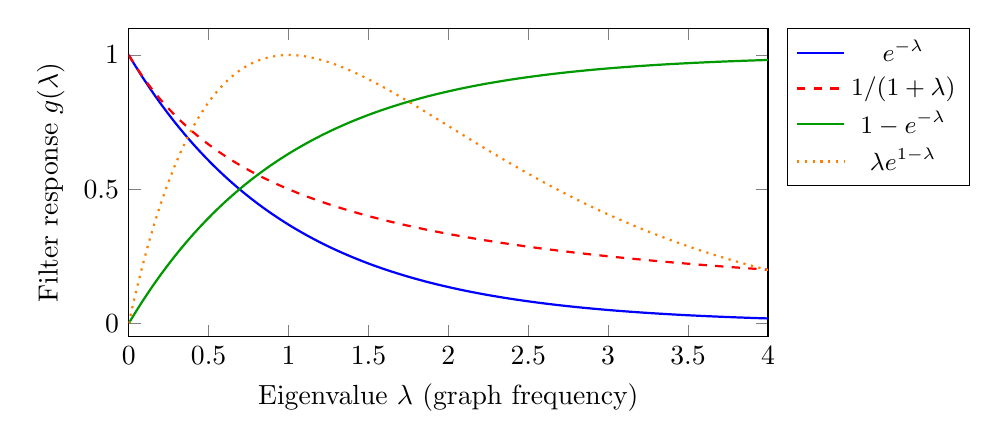
\begin{tikzpicture}
\begin{axis}[
    width=0.8\linewidth, height=5.5cm,
    xlabel={Eigenvalue $\lambda$ (graph frequency)},
    ylabel={Filter response $g(\lambda)$},
    xmin=0, xmax=4,
    ymin=-0.05, ymax=1.1,
    legend pos=outer north east,
    legend style={font=\small},
]
\addplot[thick, blue, domain=0:4, samples=100] {exp(-x)};
\addlegendentry{$e^{-\lambda}$}
\addplot[thick, red, dashed, domain=0:4, samples=100] {1/(1+x)};
\addlegendentry{$1/(1+\lambda)$}
\addplot[thick, green!60!black, domain=0:4, samples=100] {1 - exp(-x)};
\addlegendentry{$1 - e^{-\lambda}$}
\addplot[thick, orange, dotted, domain=0:4, samples=100] {x*exp(1-x)};
\addlegendentry{$\lambda e^{1-\lambda}$}
\end{axis}
\end{tikzpicture}
\caption{Frequency responses of spectral graph filters: two low-pass filters (heat kernel and regularization filter, $t=\alpha=1$), a high-pass filter and a band-pass filter.}
\label{dft-to-gnn:fig:filters}
\end{figure}

\subsection{Why polynomial filters are crucial: computational efficiency}

The full spectral convolution $\mathbf{y} = U g(\Lambda) U^\top \mathbf{x}$ requires:
\begin{enumerate}
\item Computing eigendecomposition $L = U\Lambda U^\top$: $O(N^3)$ operations.
\item Applying $U^\top$ and $U$: $O(N^2)$ each.
\end{enumerate}
For large graphs (millions of nodes), this is impossible.

However, if $g(\lambda)$ is a \emph{polynomial} of degree $K-1$:
\[
g(\lambda) = \sum_{k=0}^{K-1} \theta_k \lambda^k
\]
then:
\[
U g(\Lambda) U^\top = \sum_{k=0}^{K-1} \theta_k U\Lambda^k U^\top = \sum_{k=0}^{K-1} \theta_k L^k
\]
No eigendecomposition needed. We only need to compute $L^k \mathbf{x}$ for
$k = 0, 1, \ldots, K-1$.

\paragraph{What does $L^k \mathbf{x}$ compute?}
Recall that $(L\mathbf{x})_i = \sum_{j \sim i} A_{ij}(x_i - x_j)$ measures
local variation. Then:
\begin{itemize}
\item $L^0\mathbf{x} = \mathbf{x}$ (the signal itself).
\item $L^1\mathbf{x}$ aggregates information from immediate neighbours.
\item $L^2\mathbf{x} = L(L\mathbf{x})$ aggregates from 2-hop neighbours.
\item $L^k\mathbf{x}$ aggregates information from $k$-hop neighbours.
\end{itemize}

So polynomial filters of degree $K-1$ combine information from up to
$(K-1)$-hop neighbourhoods, with weights $\theta_k$ learned from data. The precise statement is the following.

\begin{lemma}[Polynomial filters are local]\label{dft-to-gnn:lem:local}
Let $\operatorname{dist}(i,j)$ be the shortest-path distance in $G$. Then $(L^k)_{ij} = 0$ whenever $\operatorname{dist}(i,j) > k$. Consequently, for a polynomial $g$ of degree $K-1$, $(g(L)\mathbf{x})_i$ depends only on the values $x_j$ with $\operatorname{dist}(i,j) \le K-1$.
\end{lemma}

\begin{proof}
$L_{ij} \ne 0$ only if $i = j$ or $j \sim i$. Expanding, $(L^k)_{ij} = \sum_{m_1,\ldots,m_{k-1}} L_{i m_1}L_{m_1m_2}\cdots L_{m_{k-1}j}$, and a non-zero term requires a sequence $i, m_1, \ldots, m_{k-1}, j$ in which consecutive nodes are equal or adjacent, that is a walk of length at most $k$ from $i$ to $j$. None exists when $\operatorname{dist}(i,j) > k$.
\end{proof}

The lemma is due to Hammond et al.\ (2011); it is what makes polynomial filters behave like the small kernels of a CNN rather than like a global Fourier multiplier.

\subsection{Verification: recovering classical convolution}

On the circular graph, $U = F^*/\sqrt{N}$ (the normalized DFT matrix)
and $\Lambda$ contains the eigenvalues $\lambda_k = 4\sin^2(\pi k/N)$. Since $U$ is complex, the transform is $U^*\mathbf{x}$ rather than $U^\top\mathbf{x}$.
If we choose a filter that depends on $k$ rather than $\lambda_k$, we
recover exactly the classical convolution theorem.

\begin{example}[Circular convolution as special case]
For the circular graph, let $g(\lambda_k) = H_k$ where $H_k$ is the
DFT of some filter $\mathbf{h}$. Then:
\begin{align*}
\mathbf{x} *_G g &= U \, \diag(H_0, \ldots, H_{N-1}) \, U^* \mathbf{x} \\
&= \frac{1}{\sqrt{N}} F^* \, \diag(\mathbf{H}) \,
   \frac{1}{\sqrt{N}} F \mathbf{x} \\
&= F^{-1} \, \diag(\mathbf{H}) \, F \mathbf{x} \\
&= C_h \mathbf{x} = \mathbf{x} \circledast \mathbf{h}
\end{align*}
which is exactly circular convolution.
\end{example}

\begin{pitfall}[Not every convolution is a function of $L$]
In the example, the multiplier $H_k$ is indexed by the frequency $k$, not by the eigenvalue. Because $\lambda_k = \lambda_{N-k}$, a filter of the form $g(\lambda_k)$ must satisfy $H_k = H_{N-k}$; for a real filter $\mathbf{h}$ this means $h[n] = h[-n \bmod N]$. So the spectral filters $g(L)$ of the cycle are exactly the circular convolutions with \emph{symmetric} kernels: a kernel that distinguishes left from right, such as $\mathbf{h} = (0, 1, 0, \ldots, 0)$ (a shift by one), is not of the form $g(L)$. On a general graph the loss is the same: $g(L)$ can only treat all directions within an eigenspace alike.
\end{pitfall}

\subsection{Example: applying a low-pass filter on a path graph}

Let us apply a low-pass filter $g(\lambda) = e^{-\lambda}$ to a signal
on the path graph $P_4$.

\begin{example}[Spectral convolution on $P_4$]
Consider the path graph $P_4$ with signal $\mathbf{x} = [1, 0, 0, 0]^\top$
(a unit impulse at node 0). We want to smooth this signal using a
low-pass filter $g(\lambda) = e^{-\lambda}$.

From our earlier calculation (the DCT-II basis of \cref{dft-to-gnn:thm:path-dct} with $N = 4$), the
orthonormal eigenvectors and the eigenvalues are:
\begin{align*}
\lambda_0 &= 0, \quad \mathbf{u}_0 = \tfrac{1}{2}(1, 1, 1, 1)^\top \\
\lambda_1 &= 2 - \sqrt{2} \approx 0.586, \quad \mathbf{u}_1 \approx (0.653, 0.271, -0.271, -0.653)^\top \\
\lambda_2 &= 2, \quad \mathbf{u}_2 = \tfrac{1}{2}(1, -1, -1, 1)^\top \\
\lambda_3 &= 2 + \sqrt{2} \approx 3.414, \quad \mathbf{u}_3 \approx (0.271, -0.653, 0.653, -0.271)^\top
\end{align*}
(The graph Fourier transform requires an \emph{orthonormal} basis: the vectors must be normalized.)

\emph{Step 1: graph Fourier transform.}
\[
\hat{\mathbf{x}} = U^\top \mathbf{x} =
\begin{pmatrix}
\mathbf{u}_0^\top \mathbf{x} \\
\mathbf{u}_1^\top \mathbf{x} \\
\mathbf{u}_2^\top \mathbf{x} \\
\mathbf{u}_3^\top \mathbf{x}
\end{pmatrix}
\approx
\begin{pmatrix}
0.5 \\
0.653 \\
0.5 \\
0.271
\end{pmatrix}
\]
Since $\mathbf{x}$ is the impulse at node 0, $\hat{x}_k = u_k[0]$: the impulse contains \emph{all}
frequencies, but not with equal weights (unlike the classical DFT, where an impulse has a flat spectrum,
the graph eigenvectors do not all have the same magnitude at node 0).

\emph{Step 2: apply filter in frequency domain.}
\[
g(\Lambda) = \diag(e^0, e^{-0.586}, e^{-2}, e^{-3.414})
\approx \diag(1, 0.557, 0.135, 0.033)
\]
\[
\hat{\mathbf{y}} = g(\Lambda) \hat{\mathbf{x}} \approx
\begin{pmatrix}
1 \times 0.5 \\
0.557 \times 0.653 \\
0.135 \times 0.5 \\
0.033 \times 0.271
\end{pmatrix}
\approx
\begin{pmatrix}
0.5 \\
0.364 \\
0.068 \\
0.009
\end{pmatrix}
\]

\emph{Step 3: inverse graph Fourier transform.}
\[
\mathbf{y} = U \hat{\mathbf{y}} = 0.5\mathbf{u}_0 + 0.364\mathbf{u}_1 +
0.068\mathbf{u}_2 + 0.009\mathbf{u}_3
\]
Approximately:
\[
\mathbf{y} \approx
\begin{pmatrix}
    0.25+0.238+0.034+0.002\\
    0.25+0.098-0.034-0.006\\
    0.25-0.098-0.034+0.006\\
    0.25-0.238+0.034-0.002
\end{pmatrix}
\]
\[
\mathbf{y} \approx [0.524, 0.309, 0.124, 0.044]^\top
\]
This is $e^{-L}\mathbf{x}$, the heat kernel applied to the impulse (checked numerically). Note that the
entries still sum to $1$: since $L\mathbf{1} = \mathbf{0}$, heat diffusion conserves the total ``mass'' of the
signal.

The impulse has been smoothed across the graph. The low-pass filter
attenuated high-frequency components, spreading the energy from node 0
to its neighbours.
\end{example}

%==========================================================================
\section{Application: graph convolutional networks}\label{dft-to-gnn:sec:gcn}
%==========================================================================

\subsection{The machine learning context}

In many applications, data naturally lives on graphs:
\begin{itemize}
\item Social networks: users and friendships.
\item Molecules: atoms and bonds.
\item Citation networks: papers and references.
\item Knowledge graphs: entities and relations.
\end{itemize}

We want neural networks that can process such data while respecting
the graph structure --- analogous to how CNNs process images while
respecting the grid structure.

\subsection{Spectral graph neural networks}

The spectral approach to graph convolution gives us:

\begin{definition}[Spectral graph convolutional layer]
Given input signal $\mathbf{x} \in \R^N$ and learnable filter
$g_\theta$:
\begin{equation}
\mathbf{y} = \sigma\left( U \, g_\theta(\Lambda) \, U^\top \mathbf{x}
             \right)
\end{equation}
where $\sigma$ is a nonlinearity (e.g.\ ReLU).
\end{definition}

\paragraph{Problem.} Computing the full eigendecomposition
$L = U\Lambda U^\top$ costs $O(N^3)$. For large graphs, this is
prohibitive.

\subsection{ChebNet: using Chebyshev polynomials}

We have seen that polynomial filters $g(\lambda) = \sum_{k=0}^{K-1}
\theta_k \lambda^k$ avoid eigendecomposition. ChebNet (Defferrard, Bresson and Vandergheynst, \emph{Convolutional Neural Networks on Graphs with Fast Localized Spectral Filtering}, 2016) improves on this
by using \emph{Chebyshev polynomials} instead of the standard monomial
basis.

\subsubsection{Why change the polynomial basis?}

Any polynomial of degree $K-1$ can be written either as:
\[
\sum_{k=0}^{K-1} a_k \lambda^k \quad \text{(monomial basis)}
\qquad \text{or} \qquad
\sum_{k=0}^{K-1} b_k T_k(\lambda) \quad \text{(Chebyshev basis)}
\]

These are just two different ways to parametrize the \emph{same} set
of polynomials. So why prefer Chebyshev?

\begin{enumerate}
\item \textbf{Numerical stability}: The monomials $\lambda^k$ can grow
      very large or very small, causing numerical issues. Chebyshev
      polynomials satisfy $|T_k(x)| \leq 1$ for $x \in [-1, 1]$.

\item \textbf{Efficient recurrence}: Chebyshev polynomials satisfy
      \[
      T_0(x) = 1, \quad T_1(x) = x, \quad
      T_{k+1}(x) = 2x \cdot T_k(x) - T_{k-1}(x)
      \]
      This allows computing $T_k(\tilde{L})\mathbf{x}$ recursively without
      storing or computing high powers of $L$.

\item \textbf{Orthogonality}: Chebyshev polynomials are orthogonal
      with respect to a certain weight, which can help optimization.
\end{enumerate}

\subsubsection{The rescaling step}

Chebyshev polynomials are well-behaved on $[-1, 1]$, but the eigenvalues
of $L$ lie in $[0, \lambda_{\max}]$. We therefore rescale:

\begin{equation}
\tilde{\lambda} = \frac{2\lambda}{\lambda_{\max}} - 1
\quad \in [-1, 1]
\end{equation}

Equivalently, we define the rescaled Laplacian:
\begin{equation}
\tilde{L} = \frac{2L}{\lambda_{\max}} - I
\end{equation}

The ChebNet filter is then:
\begin{equation}
\mathbf{y} = \sum_{k=0}^{K-1} \theta_k \, T_k(\tilde{L}) \, \mathbf{x}
\end{equation}

\subsubsection{Efficient computation via recurrence}

Using the Chebyshev recurrence, we compute:
\begin{align}
\bar{\mathbf{x}}_0 &= \mathbf{x} \\
\bar{\mathbf{x}}_1 &= \tilde{L} \mathbf{x} \\
\bar{\mathbf{x}}_k &= 2\tilde{L} \bar{\mathbf{x}}_{k-1} - \bar{\mathbf{x}}_{k-2}
\end{align}

Then:
\[
\mathbf{y} = \sum_{k=0}^{K-1} \theta_k \bar{\mathbf{x}}_k
\]

This requires only $K$ sparse matrix-vector multiplications with $L$,
giving complexity $O(K \cdot |E|)$ instead of $O(N^3)$.

\begin{example}[ChebNet computation on a triangle graph]
Consider a triangle graph (3 nodes, each connected to the other two)
with signal $\mathbf{x} = [1, 0, 0]^\top$ (a unit impulse at node 0).

\begin{center}
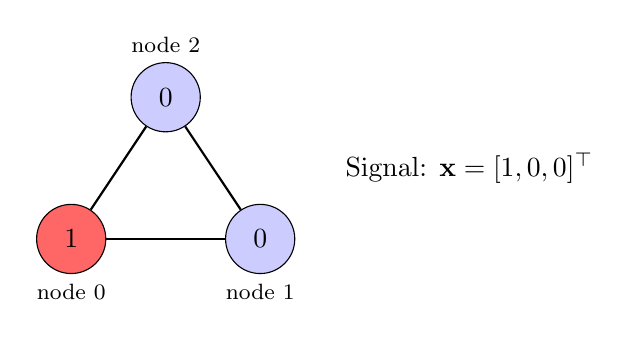
\begin{tikzpicture}[scale=1.2]
    % Nodes
    \node[circle, draw, fill=red!60, minimum size=25pt] (n0) at (0, 0) {$1$};
    \node[circle, draw, fill=blue!20, minimum size=25pt] (n1) at (2, 0) {$0$};
    \node[circle, draw, fill=blue!20, minimum size=25pt] (n2) at (1, 1.5) {$0$};

    % Edges
    \draw[thick] (n0) -- (n1);
    \draw[thick] (n1) -- (n2);
    \draw[thick] (n2) -- (n0);

    % Labels
    \node[below] at (n0.south) {\footnotesize node 0};
    \node[below] at (n1.south) {\footnotesize node 1};
    \node[above] at (n2.north) {\footnotesize node 2};

    % Signal annotation
    \node[right] at (2.8, 0.75) {Signal: $\mathbf{x} = [1, 0, 0]^\top$};
\end{tikzpicture}
\end{center}

The Laplacian is:
\[
L = \begin{pmatrix} 2 & -1 & -1 \\ -1 & 2 & -1 \\ -1 & -1 & 2 \end{pmatrix}
\]
with $\lambda_{\max} = 3$. The rescaled Laplacian is:
\[
\tilde{L} = \frac{2}{3}L - I =
\begin{pmatrix} 1/3 & -2/3 & -2/3 \\ -2/3 & 1/3 & -2/3 \\ -2/3 & -2/3 & 1/3 \end{pmatrix}
\]

For $K=3$ (degree-2 polynomial), we compute:

\emph{Step 1}: $\bar{\mathbf{x}}_0 = T_0(\tilde{L})\mathbf{x} = \mathbf{x} = [1, 0, 0]^\top$

\emph{Step 2}: $\bar{\mathbf{x}}_1 = T_1(\tilde{L})\mathbf{x} = \tilde{L}\mathbf{x} = [1/3, -2/3, -2/3]^\top$

\emph{Step 3}: $\bar{\mathbf{x}}_2 = 2\tilde{L}\bar{\mathbf{x}}_1 - \bar{\mathbf{x}}_0$. Combining the columns of $\tilde L$ with the weights $\frac13, -\frac23, -\frac23$,
\[
\tilde{L}\bar{\mathbf{x}}_1
= \tfrac{1}{3}\begin{pmatrix} 1/3 \\ -2/3 \\ -2/3 \end{pmatrix}
- \tfrac{2}{3}\begin{pmatrix} -2/3 \\ 1/3 \\ -2/3 \end{pmatrix}
- \tfrac{2}{3}\begin{pmatrix} -2/3 \\ -2/3 \\ 1/3 \end{pmatrix}
= \begin{pmatrix} 1 \\ 0 \\ 0 \end{pmatrix},
\qquad
\bar{\mathbf{x}}_2 = 2\begin{pmatrix} 1 \\ 0 \\ 0 \end{pmatrix} - \begin{pmatrix} 1 \\ 0 \\ 0 \end{pmatrix} = \begin{pmatrix} 1 \\ 0 \\ 0 \end{pmatrix}.
\]
This is no accident: the eigenvalues of $L$ are $0, 3, 3$, so those of $\tilde L$ are $-1, 1, 1$, hence $\tilde L^2 = I$ and $T_2(\tilde L) = 2\tilde L^2 - I = I$.

\emph{Step 4}: Output with learned weights $\theta_0, \theta_1, \theta_2$:
\[
\mathbf{y} = (\theta_0 + \theta_2) \begin{pmatrix} 1 \\ 0 \\ 0 \end{pmatrix}
+ \theta_1 \begin{pmatrix} 1/3 \\ -2/3 \\ -2/3 \end{pmatrix}.
\]

We computed this with two sparse matrix-vector products with $\tilde{L}$, without eigenvectors. The example also shows a limitation: a graph with only two distinct eigenvalues supports only a two-dimensional space of filters, and the third coefficient is redundant. In general a filter on a graph with $r$ distinct eigenvalues is determined by its values at those $r$ points, so polynomials of degree $r-1$ already give all spectral filters.
\end{example}

\subsection{GCN: the simplified first-order case}

The Graph Convolutional Network (GCN) of Kipf and Welling (\emph{Semi-Supervised Classification with Graph Convolutional Networks}, 2017)
simplifies ChebNet by keeping only polynomials of degree one (first-order neighbours) and making additional approximations. It uses the symmetric normalized Laplacian $L = L_{\text{sym}} = I - D^{-1/2}AD^{-1/2}$ of \cref{ch:graph-laplacians}, whose eigenvalues lie in $[0, 2]$.

Starting from a first-order Chebyshev filter ($K=2$ terms in our indexing):

\[
\mathbf{y} = \theta_0 \mathbf{x} + \theta_1 \tilde{L} \mathbf{x}
\]
where $\tilde{L} = \frac{2}{\lambda_{\max}}L - I$ is the rescaled Laplacian.

GCN makes two simplifying assumptions:
\begin{enumerate}
\item $\lambda_{\max} \approx 2$ (the upper bound of the spectrum of $L_{\text{sym}}$, attained exactly for bipartite graphs).
\item $\theta = \theta_0 = -\theta_1$ (tie the parameters).
\end{enumerate}

With these assumptions and $\lambda_{\max} = 2$, we have
$\tilde{L} = L - I$, so:
\[
\mathbf{y} = \theta \mathbf{x} - \theta(L - I)\mathbf{x}
           = \theta(2I - L)\mathbf{x}
           = \theta(I + D^{-1/2} A D^{-1/2})\mathbf{x}
\]
where $A$ is the adjacency matrix and $D$ is the degree matrix.

\subsubsection{From filter to neural network layer}

The expression $\theta(I + D^{-1/2} A D^{-1/2})\mathbf{x}$ is a spectral
filter with a single learnable parameter $\theta$. To turn this into a
useful neural network layer, we make three modifications:

\paragraph{Step 1: renormalization trick.} The term $I + D^{-1/2} A D^{-1/2}$
combines the normalized adjacency with the identity. Its eigenvalues $2 - \lambda_k$ lie in $[0, 2]$, so stacking many such layers can amplify the components with eigenvalue near $2$ and cause exploding or vanishing activations. Kipf and Welling proposed a ``renormalization trick'': instead
of adding $I$ after normalizing, add self-loops \emph{before} normalizing.
Define $\hat{A} = A + I$ (the adjacency matrix with self-loops added) and let $\hat{D}$ be the degree matrix of $\hat{A}$, that is
$\hat{D}_{ii} = \sum_j \hat{A}_{ij} = D_{ii} + 1$.
Then use $\hat{D}^{-1/2} \hat{A} \hat{D}^{-1/2}$ instead of
$I + D^{-1/2} A D^{-1/2}$. Since $\hat D^{-1/2}\hat A\hat D^{-1/2} = I - \hat L_{\text{sym}}$ for the graph with self-loops, its eigenvalues lie in $[-1, 1]$, and one checks that the self-loops keep them away from $-1$ (\cref{dft-to-gnn:exr:4}); this improves training stability.

\paragraph{Step 2: replace scalar $\theta$ with weight matrix $W$.}
Instead of a single scalar parameter, we use a learnable weight matrix
$W \in \mathbb{R}^{d \times d'}$ that transforms $d$-dimensional input
features to $d'$-dimensional output features. This allows the layer to
learn rich feature transformations.

\paragraph{Step 3: add nonlinearity.} To enable the network to learn
nonlinear functions, we apply an activation function $\sigma$ (typically
ReLU) after the linear transformation.

\emph{The final GCN layer} combines these three modifications:

\begin{equation}
H^{(l+1)} = \sigma\left( \hat{D}^{-1/2} \hat{A} \hat{D}^{-1/2}
             H^{(l)} W^{(l)} \right)
\end{equation}

where:
\begin{itemize}
    \item $H^{(l)} \in \mathbb{R}^{N \times d}$ is the matrix of node
          features at layer $l$ ($N$ nodes, $d$ features each).
    \item $W^{(l)} \in \mathbb{R}^{d \times d'}$ is the learnable weight
          matrix for layer $l$.
    \item $\sigma$ is a nonlinear activation (e.g.\ ReLU).
    \item $H^{(l+1)} \in \mathbb{R}^{N \times d'}$ is the output.
\end{itemize}

\begin{remark}[From scalars to matrices]
In the original spectral filter, each node had a scalar signal value
$x_i$, and $\theta$ was a scalar parameter. In the GCN layer:
\begin{itemize}
    \item Each node has a \emph{feature vector} $\mathbf{h}_i \in \mathbb{R}^d$,
          so we stack them into a matrix $H \in \mathbb{R}^{N \times d}$.
    \item The scalar $\theta$ becomes a \emph{weight matrix}
          $W \in \mathbb{R}^{d \times d'}$ that transforms features.
\end{itemize}
\end{remark}

\begin{example}[GCN layer on a small graph]
Consider a 4-node graph where each node has 2 features:

\begin{center}
\begin{tikzpicture}[scale=1.0]
    \node[circle, draw, fill=red!30, minimum size=25pt] (n0) at (0, 1) {0};
    \node[circle, draw, fill=green!30, minimum size=25pt] (n1) at (2, 1) {1};
    \node[circle, draw, fill=blue!30, minimum size=25pt] (n2) at (2, -0.5) {2};
    \node[circle, draw, fill=orange!30, minimum size=25pt] (n3) at (0, -0.5) {3};
    \draw[thick] (n0) -- (n1);
    \draw[thick] (n1) -- (n2);
    \draw[thick] (n2) -- (n3);
    \draw[thick] (n3) -- (n0);
    \draw[thick] (n0) -- (n2);

    % Feature annotations
    \node[right, font=\small] at (2.8, 0.8) {
        $H^{(0)} = \begin{pmatrix}
        1 & 0 \\ 0 & 1 \\ 1 & 1 \\ 0 & 0
        \end{pmatrix}$};
    \node[right, font=\small] at (2.8, -0.2) {\footnotesize (4 nodes, 2 features)};
\end{tikzpicture}
\end{center}

\emph{Step 1: compute $\hat{A}$ and $\hat{D}$.}
Adjacency matrix, without and with self-loops:
\[
A = \begin{pmatrix}
0 & 1 & 1 & 1 \\
1 & 0 & 1 & 0 \\
1 & 1 & 0 & 1 \\
1 & 0 & 1 & 0
\end{pmatrix}, \quad
\hat{A} = A + I = \begin{pmatrix}
1 & 1 & 1 & 1 \\
1 & 1 & 1 & 0 \\
1 & 1 & 1 & 1 \\
1 & 0 & 1 & 1
\end{pmatrix}
\]

Degrees: $\hat{D} = \diag(4, 3, 4, 3)$.

\emph{Step 2: compute the normalized adjacency.}
\[
\hat{D}^{-1/2} \hat{A} \hat{D}^{-1/2} =
{
\renewcommand{\arraystretch}{1.5} % Increases row height
\setlength{\arraycolsep}{4pt}    % Adjusts column width
\begin{pmatrix}
\frac{1}{4} & \frac{1}{2\sqrt{3}} & \frac{1}{4} & \frac{1}{2\sqrt{3}} \\
\frac{1}{2\sqrt{3}} & \frac{1}{3} & \frac{1}{2\sqrt{3}} & 0 \\
\frac{1}{4} & \frac{1}{2\sqrt{3}} & \frac{1}{4} & \frac{1}{2\sqrt{3}} \\
\frac{1}{2\sqrt{3}} & 0 & \frac{1}{2\sqrt{3}} & \frac{1}{3}
\end{pmatrix}
=
\begin{pmatrix}
0.25 & 0.29 & 0.25 & 0.29 \\
0.29 & 0.33 & 0.29 & 0 \\
0.25 & 0.29 & 0.25 & 0.29 \\
0.29 & 0 & 0.29 & 0.33
\end{pmatrix}
}
\]
(entries rounded to 2 decimal places)

\emph{Step 3: apply GCN layer.} With weight matrix
$W = \begin{pmatrix} 1 & 0 \\ 0 & 1 \end{pmatrix}$ (identity, for simplicity):

\[
H^{(1)} = \sigma\left( \hat{D}^{-1/2} \hat{A} \hat{D}^{-1/2} H^{(0)} W \right)
\]

First, aggregate features (before nonlinearity):
\[
\hat{D}^{-1/2} \hat{A} \hat{D}^{-1/2} H^{(0)} =
\begin{pmatrix}
0.25 + 0.25 & 0.29 + 0.25 \\
0.29 + 0.29 & 0.33 + 0.29 \\
0.25 + 0.25 & 0.29 + 0.25 \\
0.29 + 0.29 & 0.29
\end{pmatrix}
= \begin{pmatrix}
0.50 & 0.54 \\
0.58 & 0.62 \\
0.50 & 0.54 \\
0.58 & 0.29
\end{pmatrix}
\]

Each row is now a weighted average of that node's features and its
neighbours' features. Applying ReLU (all values positive, so unchanged):
\[
H^{(1)} = \begin{pmatrix}
0.50 & 0.54 \\
0.58 & 0.62 \\
0.50 & 0.54 \\
0.58 & 0.29
\end{pmatrix}
\]

(Row $i$ of the propagation matrix uses the entries of row $i$ only: for node $2$ these are $\frac14, \frac1{2\sqrt3}, \frac14, \frac1{2\sqrt3}$, the same as for node $0$.) Nodes $0$ and $2$ end up with identical features although their inputs $(1,0)$ and $(1,1)$ differ: each is adjacent to all other nodes, so their neighbourhoods with self-loops coincide ($\{0,1,2,3\}$), and so do their rows of $\hat D^{-1/2}\hat A\hat D^{-1/2}$. A GCN layer cannot separate nodes with the same closed neighbourhood; repeated layers blur more and more nodes together, which is the over-smoothing discussed below.
\end{example}

\subsubsection{Interpretation of GCN}

The GCN layer can be interpreted as:
\begin{enumerate}
\item \textbf{Feature transformation}: Multiply by $W$ to learn
      new feature representations.
\item \textbf{Neighbourhood aggregation}: Multiply by
      $\hat{D}^{-1/2} \hat{A} \hat{D}^{-1/2}$ to average each node's
      features with its neighbours' features.
\item \textbf{Nonlinearity}: Apply $\sigma$ (e.g.\ ReLU) to enable
      nonlinear decision boundaries.
\end{enumerate}

This simple formulation has proven remarkably effective in practice and
forms the basis for many modern GNN architectures.

\subsection{Summary: the spectral foundation of GNNs}

\begin{center}
\resizebox{\linewidth}{!}{%
\begin{tikzpicture}[node distance=2.3cm, auto,
    block/.style={rectangle, draw, fill=blue!10, align=center,
                  text width=6.5em, text centered, minimum height=2.5em,
                  rounded corners=3pt},
    arrow/.style={->, >=stealth, thick, align=center, font=\footnotesize}]

    \node[block] (dft) {DFT on\\the cycle};
    \node[block, right=of dft] (gft) {Graph Fourier\\transform};
    \node[block, right=of gft] (spec) {Spectral\\convolution};
    \node[block, right=of spec] (cheb) {ChebNet\\(degree $K$)};
    \node[block, right=of cheb] (gcn) {GCN\\($K = 1$)};

    \draw[arrow] (dft) -- node[above] {Generalize} (gft);
    \draw[arrow] (gft) -- node[above] {Define} (spec);
    \draw[arrow] (spec) -- node[above] {Polynomial\\filter} (cheb);
    \draw[arrow] (cheb) -- node[above] {Simplify} (gcn);

    \node[below=0.3cm of dft] {\footnotesize Basis: $e^{2\pi i kn/N}$};
    \node[below=0.3cm of gft] {\footnotesize Basis: eigenvectors of $L$};
    \node[below=0.3cm of spec] {\footnotesize $U g(\Lambda) U^\top$};
    \node[below=0.3cm of cheb] {\footnotesize $\sum \theta_k T_k(\tilde{L})$};
    \node[below=0.3cm of gcn] {\footnotesize $\hat{D}^{-1/2}\hat{A}\hat{D}^{-1/2}$};

    \node[below=1.2cm of dft] {\footnotesize $O(N \log N)$};
    \node[below=1.2cm of gft] {\footnotesize $O(N^3)$ (eigen)};
    \node[below=1.2cm of spec] {\footnotesize $O(N^2)$};
    \node[below=1.2cm of cheb] {\footnotesize $O(K|E|)$};
    \node[below=1.2cm of gcn] {\footnotesize $O(|E|)$};

\end{tikzpicture}%
}
\end{center}

\paragraph{Key insight.} The evolution from DFT to GCN shows a trade-off between
mathematical elegance and computational efficiency:
\begin{itemize}
\item \textbf{DFT/Spectral}: Theoretically elegant but computationally expensive.
\item \textbf{ChebNet}: Good balance between theory and computation.
\item \textbf{GCN}: Extremely efficient but with theoretical approximations.
\end{itemize}

This progression mirrors the development of CNNs: from Fourier-based filtering
to efficient local convolutions with learnable filters.

%==========================================================================
\section{Limitations of the spectral approach}
%==========================================================================

The spectral approach to graph analysis is mathematically elegant, but
it has important limitations that we must understand. Recognizing these
limitations motivates the more general framework of message passing.

\subsection{The circular graph is special}

Recall that for the circular graph, the DFT basis emerged as
eigenvectors of the Laplacian because of \emph{translational
symmetry}: every node ``looks the same'' as every other node. This is
a very special property.

\begin{remark}[Spectral convolution is a definition, not a theorem]
For the circular graph, we \emph{proved} that convolution equals
multiplication in the Fourier domain (the convolution theorem). For
general graphs, we \emph{defined} convolution as multiplication in
the spectral domain.

This is an important distinction:
\begin{itemize}
    \item \textbf{Circle}: Convolution theorem is a \emph{theorem}
          (forced by shift-invariance).
    \item \textbf{General graph}: Spectral convolution is a
          \emph{definition} (motivated by analogy).
\end{itemize}

The definition is useful because Laplacian eigenvectors still capture
``smoothness'' (low $\lambda$ = smooth, high $\lambda$ = rough), but
there is no deeper theorem forcing this choice.
\end{remark}

\subsection{Path graph vs.\ circular graph}

Even for simple graphs, the structure fundamentally changes the
eigenvectors.

\begin{example}[Path graph has different eigenvectors]
Consider the path graph $P_4$: four nodes in a line with no wrap-around.

\begin{center}
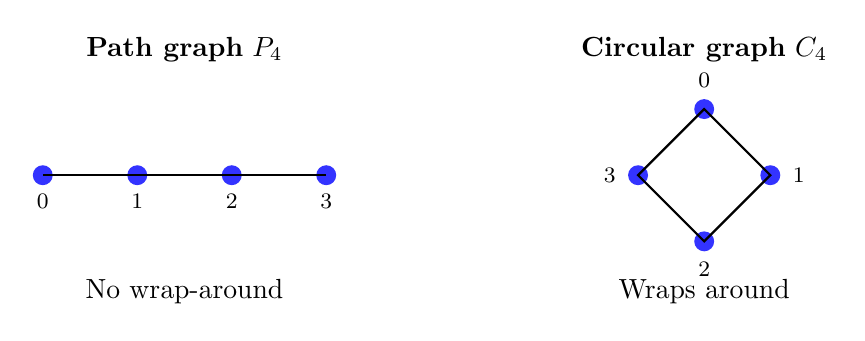
\begin{tikzpicture}[scale=1.2]
    % Path graph
    \node[above] at (1.5, 1.1) {\textbf{Path graph} $P_4$};
    \foreach \i in {0,...,3} {
        \fill[blue!80] (\i, 0) circle (3pt);
        \node[below] at (\i, -0.1) {\footnotesize $\i$};
    }
    \draw[thick] (0,0) -- (1,0) -- (2,0) -- (3,0);
    \node[below] at (1.5, -1) {No wrap-around};

    % Circular graph
    \node[above] at (7, 1.1) {\textbf{Circular graph} $C_4$};
    \foreach \i in {0,...,3} {
        \pgfmathsetmacro{\angle}{90 - \i*90}
        \fill[blue!80] ({7 + 0.7*cos(\angle)}, {0.7*sin(\angle)}) circle (3pt);
        \node at ({7 + 1.0*cos(\angle)}, {1.0*sin(\angle)}) {\footnotesize $\i$};
    }
    \draw[thick] ({7 + 0.7*cos(90)}, {0.7*sin(90)}) --
                 ({7 + 0.7*cos(0)}, {0.7*sin(0)}) --
                 ({7 + 0.7*cos(-90)}, {0.7*sin(-90)}) --
                 ({7 + 0.7*cos(180)}, {0.7*sin(180)}) -- cycle;
    \node[below] at (7, -1) {Wraps around};
\end{tikzpicture}
\end{center}

The Laplacians are different:
\[
L_{\text{path}} = \begin{pmatrix}
1 & -1 & 0 & 0 \\
-1 & 2 & -1 & 0 \\
0 & -1 & 2 & -1 \\
0 & 0 & -1 & 1
\end{pmatrix}
\quad \text{vs.} \quad
L_{\text{circle}} = \begin{pmatrix}
2 & -1 & 0 & -1 \\
-1 & 2 & -1 & 0 \\
0 & -1 & 2 & -1 \\
-1 & 0 & -1 & 2
\end{pmatrix}
\]

Key differences:
\begin{itemize}
    \item Path: endpoints have degree 1, interior nodes have degree 2.
    \item Circle: all nodes have degree 2 (perfect symmetry).
\end{itemize}

\emph{Consequence}: The eigenvectors of the path graph are
\emph{not} complex exponentials. They are related to the
\emph{Discrete Cosine Transform (DCT)}, not the DFT:
\[
u_k[n] \propto \cos\left(\frac{\pi k (n + \frac{1}{2})}{N}\right)
\]

The boundary conditions fundamentally change the eigenvectors. See
\cref{dft-to-gnn:app:dct-path} for a detailed derivation.
\end{example}

\subsection{Directed graphs: symmetry breaks down}

A more serious limitation arises with directed graphs.

\begin{definition}[Directed graph]
In a \emph{directed graph}, edges have direction: an edge from $i$
to $j$ does not imply an edge from $j$ to $i$. The adjacency matrix
satisfies $A_{ij} \neq A_{ji}$ in general.
\end{definition}

\begin{figure}[H]
\centering
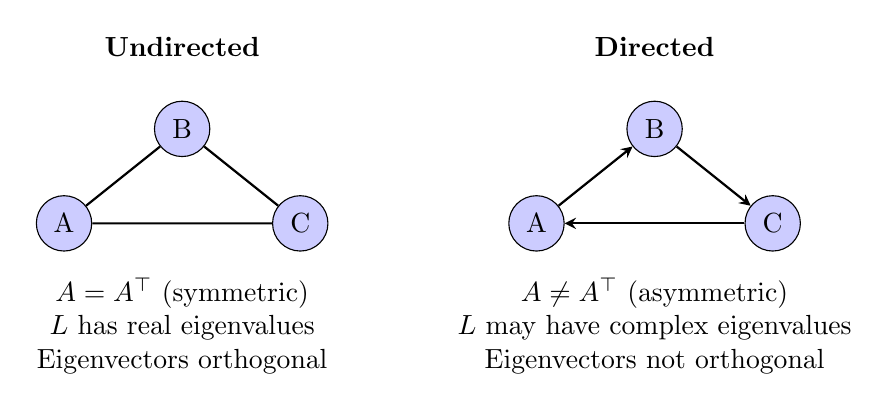
\begin{tikzpicture}[scale=1.0,
    node/.style={circle, draw, fill=blue!20, minimum size=20pt},
    arrow/.style={->, >=stealth, thick}]

    % Undirected graph
    \node[above] at (1.5, 2) {\textbf{Undirected}};
    \node[node] (a1) at (0, 0) {A};
    \node[node] (b1) at (1.5, 1.2) {B};
    \node[node] (c1) at (3, 0) {C};
    \draw[thick] (a1) -- (b1) -- (c1) -- (a1);

    \node[align=center] at (1.5, -1.3) {$A = A^\top$ (symmetric)\\
          $L$ has real eigenvalues\\
          Eigenvectors orthogonal};

    % Directed graph
    \node[above] at (7.5, 2) {\textbf{Directed}};
    \node[node] (a2) at (6, 0) {A};
    \node[node] (b2) at (7.5, 1.2) {B};
    \node[node] (c2) at (9, 0) {C};
    \draw[arrow] (a2) -- (b2);
    \draw[arrow] (b2) -- (c2);
    \draw[arrow] (c2) -- (a2);

    \node[align=center] at (7.5, -1.3) {$A \neq A^\top$ (asymmetric)\\
          $L$ may have complex eigenvalues\\
          Eigenvectors not orthogonal};
\end{tikzpicture}
\caption{Directed graphs break the symmetry that spectral methods
         rely on.}
\end{figure}

For directed graphs:
\begin{enumerate}
    \item The Laplacian $L = D - A$ is \emph{not symmetric}.
    \item Eigenvalues can be \emph{complex numbers}.
    \item Eigenvectors are \emph{not orthogonal} (left and right
          eigenvectors differ).
    \item The matrix may not even be \emph{diagonalizable}.
\end{enumerate}

This breaks the entire spectral framework:
\begin{itemize}
    \item No real ``frequencies'' to interpret.
    \item No orthonormal basis for a ``Fourier transform''.
    \item The quadratic form $\mathbf{x}^\top L \mathbf{x}$ loses its
          meaning as ``smoothness''.
\end{itemize}

\begin{example}[A simple directed graph]
Consider a directed 3-cycle: $0 \to 1 \to 2 \to 0$.

\begin{center}
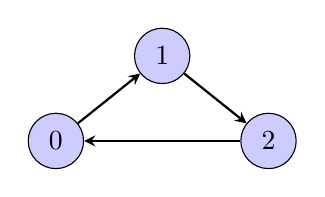
\begin{tikzpicture}[scale=0.9,
    node/.style={circle, draw, fill=blue!20, minimum size=20pt},
    arrow/.style={->, >=stealth, thick}]
    \node[node] (n0) at (0, 0) {0};
    \node[node] (n1) at (1.5, 1.2) {1};
    \node[node] (n2) at (3, 0) {2};
    \draw[arrow] (n0) -- (n1);
    \draw[arrow] (n1) -- (n2);
    \draw[arrow] (n2) -- (n0);
\end{tikzpicture}
\end{center}

\[
A = \begin{pmatrix}
0 & 1 & 0 \\
0 & 0 & 1 \\
1 & 0 & 0
\end{pmatrix}, \quad
D = \begin{pmatrix}
1 & 0 & 0 \\
0 & 1 & 0 \\
0 & 0 & 1
\end{pmatrix}, \quad
L = D - A = \begin{pmatrix}
1 & -1 & 0 \\
0 & 1 & -1 \\
-1 & 0 & 1
\end{pmatrix}
\]

The eigenvalues of $L$ are:
\[
\lambda = 0, \quad \frac{3}{2} + \frac{\sqrt{3}}{2}i, \quad
\frac{3}{2} - \frac{\sqrt{3}}{2}i
\]

Two of them are complex, so they cannot be ordered as ``frequencies''. This $L = I - A$ is still a circulant matrix, hence normal, and the complex DFT vectors are an orthonormal basis of eigenvectors; the directed cycle keeps its translation symmetry. Without that symmetry things are worse. For the directed path $0\to1\to2$, with out-degrees $D = \diag(1,1,0)$,
\[
L = \begin{pmatrix} 1 & -1 & 0 \\ 0 & 1 & -1 \\ 0 & 0 & 0 \end{pmatrix}
\]
has eigenvalues $1, 1, 0$, but $L - I$ has rank $2$, so the eigenvalue $1$ has a one-dimensional eigenspace: $L$ is not diagonalizable, and there is no eigenbasis at all in which to define a Fourier transform.
\end{example}

\subsection{Approaches for directed graphs}

Several approaches exist, but none are as clean as the undirected case:

\begin{enumerate}
    \item \textbf{Symmetrization}: Replace $A$ with
          $\frac{1}{2}(A + A^\top)$

          \emph{Problem}: Loses directional information entirely.

    \item \textbf{Magnetic Laplacian}: Encode direction as complex
          phases $e^{i\theta_{ij}}$ on edges, keeping the matrix
          Hermitian

          \emph{Advantage}: Eigenvalues stay real

          \emph{Problem}: How to choose the phases $\theta_{ij}$?

    \item \textbf{Random walk Laplacian}: Use $L_{\text{rw}} = I - D^{-1}A$

          \emph{Problem}: Still not symmetric.

    \item \textbf{Abandon spectral methods}: Use spatial/message-passing
          approaches instead (see next section).
\end{enumerate}

\subsection{Computational cost}

Even for undirected graphs, spectral methods have a practical problem:

\begin{center}
\begin{tabular}{lcc}
\toprule
Operation & Spectral & Spatial (1-hop) \\
\midrule
Eigendecomposition of $L$ & $O(N^3)$ & Not needed \\
Storing eigenvectors $U$ & $O(N^2)$ & Not needed \\
One convolution layer & $O(N^2)$ & $O(|E|)$ \\
\bottomrule
\end{tabular}
\end{center}

For large graphs (social networks with millions of nodes), $O(N^3)$
eigendecomposition is completely infeasible. This motivated polynomial
approximations (ChebNet, GCN), but these are really \emph{spatial}
methods in disguise --- they aggregate information from neighbours without
ever computing eigenvectors.

%==========================================================================
\section{Message passing: the general framework}
%==========================================================================

Given the limitations of spectral methods, we now introduce
\emph{message passing} (Gilmer et al., \emph{Neural Message Passing for Quantum Chemistry}, 2017), a more general framework
that works on any graph, including directed and heterogeneous graphs.

\subsection{The key insight}

The polynomial approximations (ChebNet, GCN) suggest a pattern: instead
of working in the spectral domain, we can directly aggregate information
from neighbours. This is the essence of \emph{spatial} or
\emph{message passing} methods.

\begin{keyidea}
Instead of transforming to a global
frequency domain, each node collects information from its local
neighbourhood and updates its representation accordingly.
\end{keyidea}

\subsection{The message passing paradigm}

\begin{definition}[Message passing neural network]
A \emph{Message Passing Neural Network (MPNN)} updates node
representations through three steps:

\begin{enumerate}
    \item \textbf{Message}: Each neighbour $j$ creates a message to send
          to node $i$.
    \item \textbf{Aggregate}: Node $i$ aggregates all incoming messages.
    \item \textbf{Update}: Node $i$ updates its representation based on
          the aggregated messages.
\end{enumerate}

Formally, for node $i$ at layer $l$:
\begin{equation}
\boxed{
h_i^{(l+1)} = \phi\left( h_i^{(l)},
    \bigoplus_{j \in \mathcal{N}(i)} \psi(h_i^{(l)}, h_j^{(l)}, e_{ji})
    \right)
}
\end{equation}
where:
\begin{itemize}
    \item $h_i^{(l)}$ = representation of node $i$ at layer $l$.
    \item $\mathcal{N}(i)$ = neighbours of node $i$ (can be in-neighbours
          for directed graphs).
    \item $\psi$ = \emph{message function} (creates messages).
    \item $\bigoplus$ = \emph{aggregation function} (sum, mean, max,
          attention, \ldots).
    \item $\phi$ = \emph{update function} (combines old state with
          aggregated messages).
    \item $e_{ji}$ = edge features from $j$ to $i$ (optional).
\end{itemize}
\end{definition}

\begin{figure}[H]
\centering
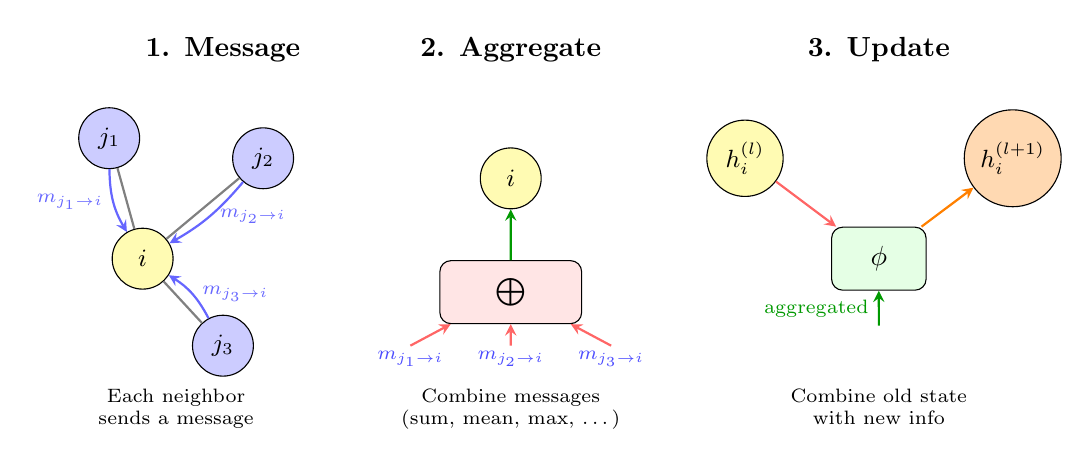
\begin{tikzpicture}[scale=0.85,
    node/.style={circle, draw, minimum size=22pt, font=\small},
    msg/.style={->, >=stealth, thick, blue!60},
    agg/.style={->, >=stealth, thick, red!60}]

    % Step 1: Message
    \node[above, font=\bfseries] at (1.2, 2.8) {1. Message};
    \node[node, fill=yellow!30] (a1) at (0, 0) {$i$};
    \node[node, fill=blue!20] (b1) at (-0.5, 1.8) {$j_1$};
    \node[node, fill=blue!20] (c1) at (1.8, 1.5) {$j_2$};
    \node[node, fill=blue!20] (d1) at (1.2, -1.3) {$j_3$};

    \draw[thick, gray] (a1) -- (b1);
    \draw[thick, gray] (a1) -- (c1);
    \draw[thick, gray] (a1) -- (d1);

    \draw[msg, bend right=15] (b1) to
        node[left, font=\scriptsize] {$m_{j_1 \to i}$} (a1);
    \draw[msg, bend left=10] (c1) to
        node[right, font=\scriptsize] {$m_{j_2 \to i}$} (a1);
    \draw[msg, bend right=15] (d1) to
        node[right, font=\scriptsize] {$m_{j_3 \to i}$} (a1);

    \node[below, font=\scriptsize, align=center] at (0.5, -1.8)
        {Each neighbor\\sends a message};

    % Step 2: Aggregate
    \node[above, font=\bfseries] at (5.5, 2.8) {2. Aggregate};
    \node[node, fill=yellow!30] (a2) at (5.5, 1.2) {$i$};
    \node[draw, rounded corners, fill=red!10,
          minimum width=1.8cm, minimum height=0.8cm]
        (agg) at (5.5, -0.5) {$\bigoplus$};

    \node[font=\scriptsize, blue!70] at (4.0, -1.5) {$m_{j_1 \to i}$};
    \node[font=\scriptsize, blue!70] at (5.5, -1.5) {$m_{j_2 \to i}$};
    \node[font=\scriptsize, blue!70] at (7.0, -1.5) {$m_{j_3 \to i}$};

    \draw[agg] (4.0, -1.3) -- (agg);
    \draw[agg] (5.5, -1.3) -- (agg);
    \draw[agg] (7.0, -1.3) -- (agg);
    \draw[agg, green!60!black, thick] (agg) -- (a2);

    \node[below, font=\scriptsize, align=center] at (5.5, -1.8)
        {Combine messages\\(sum, mean, max, \ldots)};

    % Step 3: Update
    \node[above, font=\bfseries] at (11, 2.8) {3. Update};
    \node[node, fill=yellow!30] (a3old) at (9, 1.5) {$h_i^{(l)}$};
    \node[draw, rounded corners, fill=green!10,
          minimum width=1.2cm, minimum height=0.8cm]
        (upd) at (11, 0.0) {$\phi$};
    \node[node, fill=orange!30] (a3new) at (13, 1.5) {$h_i^{(l+1)}$};

    \draw[agg] (a3old) -- (upd);
    \draw[agg, green!60!black] (11, -1.0) -- (upd)
        node[left, midway, font=\scriptsize] {aggregated};
    \draw[agg, orange] (upd) -- (a3new);

    \node[below, font=\scriptsize, align=center] at (11, -1.8)
        {Combine old state\\with new info};

\end{tikzpicture}
\caption{The three steps of message passing: (1) neighbours create
         messages, (2) messages are aggregated, (3) node updates
         its representation.}
\end{figure}

\subsection{Why message passing is more general}

Message passing has several advantages over spectral methods:

\begin{center}
\begin{tabular}{lcc}
\toprule
Property & Spectral & Message passing \\
\midrule
Directed graphs & \color{red}\ding{55} & \color{green!60!black}\ding{51} \\
Edge features & \color{red}\ding{55} & \color{green!60!black}\ding{51} \\
Node-specific transforms & \color{red}\ding{55} &
    \color{green!60!black}\ding{51} \\
Heterogeneous graphs & \color{red}\ding{55} &
    \color{green!60!black}\ding{51} \\
Scalability & $O(N^3)$ or $O(N^2)$ & $O(|E|)$ \\
Inductive learning & \color{red}\ding{55} &
    \color{green!60!black}\ding{51} \\
\bottomrule
\end{tabular}
\end{center}

\emph{Inductive learning} deserves special mention: spectral methods
require the eigenvectors $U$, which are specific to a particular graph.
If the graph changes (new nodes added), we must recompute $U$. Message
passing methods learn local rules that generalize to new, unseen graphs.

\subsection{Three flavours of GNN layers}

The vast majority of GNN architectures can be categorized into three
``flavours'' based on how they compute messages from neighbours (Bronstein et al., \emph{Geometric Deep Learning: Grids, Groups, Graphs, Geodesics, and Gauges}, 2021):

\begin{figure}[H]
\centering
\resizebox{\linewidth}{!}{%
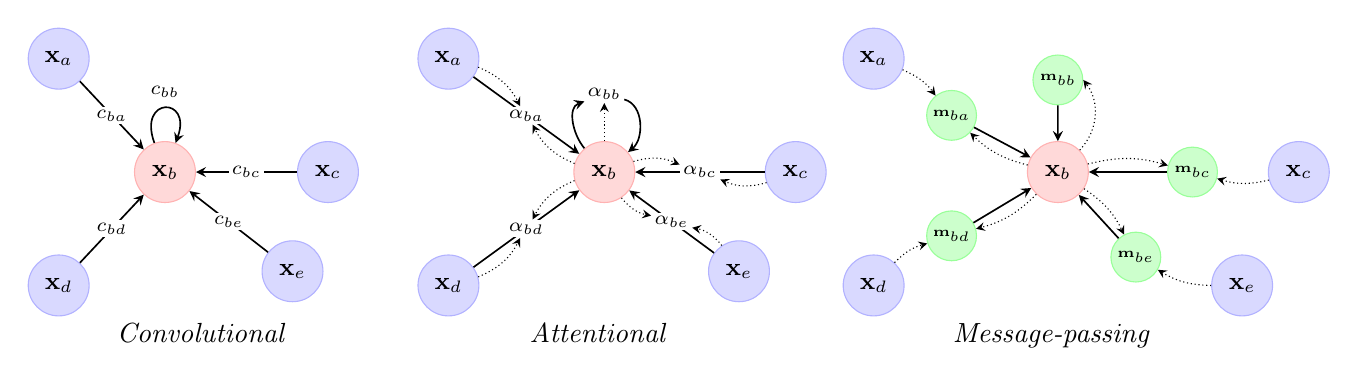
\begin{tikzpicture}[scale=0.9,
    node/.style={circle, draw=blue!30, fill=blue!15, minimum size=22pt,
    font=\bfseries\small, inner sep=1pt},
    centernode/.style={circle, draw=red!30, fill=red!15, minimum size=22pt,
    font=\bfseries\small, inner sep=1pt},
    msgnode/.style={circle, draw=green!40, fill=green!20, minimum size=18pt,
    font=\bfseries\tiny, inner sep=0.5pt},
    arrow/.style={->, >=stealth, semithick},
    dottedarrow/.style={->, >=stealth, thin, densely dotted},
    labelstyle/.style={font=\scriptsize, fill=white, inner sep=1pt}]

    % ========== Convolutional ==========
    \begin{scope}[shift={(0,0)}]
        \node[centernode] (b1) at (0, 1.2) {$\mathbf{x}_b$};
        \node[node] (a1) at (-1.5, 2.8) {$\mathbf{x}_a$};
        \node[node] (c1) at (2.3, 1.2) {$\mathbf{x}_c$};
        \node[node] (d1) at (-1.5, -0.4) {$\mathbf{x}_d$};
        \node[node] (e1) at (1.8, -0.2) {$\mathbf{x}_e$};

        \foreach \n/\lbl in {a1/c_{ba}, c1/c_{bc}, d1/c_{bd}, e1/c_{be}}
            \draw[arrow] (\n) -- (b1) node[midway, labelstyle] {$\lbl$};

        \draw[arrow] (b1) to[out=110, in=70, looseness=6] node[above, font=\scriptsize] {$c_{bb}$} (b1);
        \node[below] at (0.5, -0.8) {\itshape Convolutional};
    \end{scope}

    % ========== Attentional ==========
    \begin{scope}[shift={(5,0)}]
        \node[centernode] (b2) at (1.2, 1.2) {$\mathbf{x}_b$};
        \node[node] (a2) at (-1, 2.8) {$\mathbf{x}_a$};
        \node[node] (c2) at (3.9, 1.2) {$\mathbf{x}_c$};
        \node[node] (d2) at (-1, -0.4) {$\mathbf{x}_d$};
        \node[node] (e2) at (3.1, -0.2) {$\mathbf{x}_e$};

        \foreach \n/\lbl/\bndS/\bndN in {a2/\alpha_{ba}/20/20, c2/\alpha_{bc}/20/20, d2/\alpha_{bd}/-20/-20, e2/\alpha_{be}/-20/-20} {
            % Main flow arrow
            \draw[arrow] (\n) -- (b2) node (L-\n) [midway, labelstyle] {$\lbl$};
            % Dotted dependencies: from neighbor to alpha, and from center to alpha
            \draw[dottedarrow] (\n) to[bend left={\bndN}] (L-\n);
            \draw[dottedarrow] (b2) to[bend left={\bndS}] (L-\n);
        }

        % Self-loop with dependency
        \node (L-bb) at (1.2, 2.3) [labelstyle] {$\alpha_{bb}$};
        \draw[arrow] (b2) to[out=130, in=200, looseness=1] (L-bb);
        \draw[arrow] (L-bb) to[out=-15, in=40, looseness=1] (b2);
        \draw[dottedarrow] (b2) -- (L-bb);

        \node[below] at (1.1, -0.8) {\itshape Attentional};
    \end{scope}

    % ========== Message-passing ==========
    \begin{scope}[shift={(10,0)}]
        \node[centernode] (b3) at (2.6, 1.2) {$\mathbf{x}_b$};
        \node[node] (a3) at (0, 2.8) {$\mathbf{x}_a$};
        \node[node] (c3) at (6, 1.2) {$\mathbf{x}_c$};
        \node[node] (d3) at (0, -0.4) {$\mathbf{x}_d$};
        \node[node] (e3) at (5.2, -0.4) {$\mathbf{x}_e$};

        \node[msgnode] (ma) at (1.1, 2.0) {$\mathbf{m}_{ba}$};
        \node[msgnode] (mc) at (4.5, 1.2) {$\mathbf{m}_{bc}$};
        \node[msgnode] (md) at (1.1, 0.3) {$\mathbf{m}_{bd}$};
        \node[msgnode] (me) at (3.7, 0) {$\mathbf{m}_{be}$};
        \node[msgnode] (mb) at (2.6, 2.5) {$\mathbf{m}_{bb}$};

        \foreach \m/\src in {ma/a3, mc/c3, md/d3, me/e3} {
            \draw[arrow] (\m) -- (b3);
            \draw[dottedarrow] (\src) to[bend left=15] (\m);
            \draw[dottedarrow] (b3) to[bend left=15] (\m);
        }

        \draw[arrow] (mb) -- (b3);
        \draw[dottedarrow] (b3.north east) to[bend right=40] (mb.east);

        \node[below] at (2.5, -0.8) {\itshape Message-passing};
    \end{scope}
\end{tikzpicture}%
}
\caption{Three flavours of GNN layers (adapted from Bronstein et al., 2021),
         showing the dataflow for updating node $b$ from its neighbourhood.
         Left: Convolutional --- sender node features are multiplied
         by constant weights $c_{uv}$ from the graph structure.
         Middle: Attentional --- weights $\alpha_{uv} = a(\mathbf{x}_u, \mathbf{x}_v)$
         are implicitly computed via attention (dotted arrows show the
         receiver attending to senders).
         Right: Message-passing --- vector messages
         $\mathbf{m}_{uv} = \psi(\mathbf{x}_u, \mathbf{x}_v)$ are computed
         based on both sender and receiver (dotted arrows), then aggregated
         (solid arrows).}
\label{dft-to-gnn:fig:three-flavours}
\end{figure}


\begin{enumerate}
    \item \textbf{Convolutional} (e.g.\ GCN): Messages are scaled by
          fixed coefficients $c_{uv}$ that depend only on graph structure:
          \[
          h_u = \phi\left(x_u, \bigoplus_{v \in \mathcal{N}(u)} c_{uv} \, \psi(x_v)\right)
          \]

    \item \textbf{Attentional} (e.g.\ GAT): Coefficients are computed
          dynamically via an attention mechanism:
          \[
          h_u = \phi\left(x_u, \bigoplus_{v \in \mathcal{N}(u)}
              a(x_u, x_v) \, \psi(x_v)\right)
          \]

    \item \textbf{Message-passing} (general): Full vector messages are
          computed based on both sender and receiver:
          \[
          h_u = \phi\left(x_u, \bigoplus_{v \in \mathcal{N}(u)}
              \psi(x_u, x_v)\right)
          \]
\end{enumerate}

These form a hierarchy of expressiveness:
\emph{convolutional $\subset$ attentional $\subset$ message-passing}.
Attentional GNNs can represent convolutional GNNs by setting
$a(x_u, x_v) = c_{uv}$, and message-passing generalizes both by allowing
vector-valued (rather than scalar) interactions between nodes.

\subsection{Example: GCN as message passing}

Let us see how the GCN layer fits into the message passing framework.

\begin{example}[GCN layer]
Recall from \cref{dft-to-gnn:sec:gcn} that the GCN layer in matrix form is:
\[
H^{(l+1)} = \sigma\left( \hat{D}^{-1/2} \hat{A} \hat{D}^{-1/2}
             H^{(l)} W^{(l)} \right)
\]
where $\hat{A} = A + I$ (adjacency with self-loops), $\hat{D}$ is
its degree matrix, and $H^{(l)} \in \mathbb{R}^{N \times d}$ has node
features as rows.

\emph{Deriving the per-node form.} The $(i,j)$ entry of
$\hat{D}^{-1/2} \hat{A} \hat{D}^{-1/2}$ is:
\[
\left(\hat{D}^{-1/2} \hat{A} \hat{D}^{-1/2}\right)_{ij} =
\frac{\hat{A}_{ij}}{\sqrt{\hat{d}_i}\sqrt{\hat{d}_j}}
\]
where $\hat{d}_i = d_i + 1$ is the degree including the self-loop.

Since $\hat{A}_{ij} = 1$ if $j \in \mathcal{N}(i) \cup \{i\}$ and $0$
otherwise, the $i$-th row of $\hat{D}^{-1/2} \hat{A} \hat{D}^{-1/2} H^{(l)}$ is:
\[
\sum_{j \in \mathcal{N}(i) \cup \{i\}}
    \frac{1}{\sqrt{\hat{d}_i}\sqrt{\hat{d}_j}} h_j^{(l)}
\]
where $h_j^{(l)}$ is the $j$-th row of $H^{(l)}$ (a row vector).

Multiplying by $W^{(l)}$ on the right and applying $\sigma$, the
updated feature vector for node $i$ is:
\[
h_i^{(l+1)} = \sigma\left( \sum_{j \in \mathcal{N}(i) \cup \{i\}}
    \frac{1}{\sqrt{d_i + 1}\sqrt{d_j + 1}} h_j^{(l)} W^{(l)} \right)
\]

\emph{In message passing terms:}
\begin{itemize}
    \item \textbf{Message from $j$ to $i$}:
          $m_{j \to i} = \frac{1}{\sqrt{d_i+1}\sqrt{d_j+1}} h_j W$.
    \item \textbf{Aggregation}: $\bigoplus = \sum$ (summation).
    \item \textbf{Update}: $\phi = \sigma$ (nonlinearity, e.g.\ ReLU).
\end{itemize}

The normalization $\frac{1}{\sqrt{d_i+1}\sqrt{d_j+1}}$ comes from the
symmetric normalized adjacency and prevents high-degree nodes from
dominating the aggregation.
\end{example}

\subsection{Example: GraphSAGE}

GraphSAGE (Hamilton, Ying and Leskovec, \emph{Inductive Representation Learning on Large Graphs}, 2017; ``sample and aggregate'') is a popular message passing variant:

\begin{example}[GraphSAGE layer]
\[
h_i^{(l+1)} = \sigma\left(
    \text{CONCAT}\left(
    h_i^{(l)}, \text{AGG}(\{h_j^{(l)} : j \in \mathcal{N}(i)\})
    \right) W^{(l)} \right)
\]

Key features:
\begin{itemize}
    \item \textbf{Message}: Identity (just use neighbour features).
    \item \textbf{Aggregation}: Mean, max-pooling, or LSTM.
    \item \textbf{Update}: Concatenate self with aggregated neighbours,
          then linear transform by $W$.
\end{itemize}

The concatenation explicitly separates ``self'' information from
``neighbour'' information.
\end{example}

\subsection{Example: graph attention networks (GAT)}

The graph attention network (GAT) of Veličković et al.\ (\emph{Graph Attention Networks}, 2018) introduces learnable attention weights:

\begin{example}[GAT layer]
\[
h_i^{(l+1)} = \sigma\left( \sum_{j \in \mathcal{N}(i) \cup \{i\}}
    \alpha_{ij} \, h_j^{(l)} W \right)
\]

where the attention coefficients $\alpha_{ij}$ are computed as:
\[
\alpha_{ij} = \frac{\exp\bigl(\text{LeakyReLU}(
    [h_i W \| h_j W] \, \mathbf{a})\bigr)}
    {\sum_{k \in \mathcal{N}(i) \cup \{i\}} \exp\bigl(\text{LeakyReLU}(
    [h_i W \| h_k W] \, \mathbf{a})\bigr)}
\]

Here $[h_i W \| h_j W]$ denotes concatenation of the two transformed
row vectors (giving a row vector of size $2d'$), and
$\mathbf{a} \in \mathbb{R}^{2d'}$ is a learnable attention vector.

Key features:
\begin{itemize}
    \item \textbf{Message}: Weighted by learned attention $\alpha_{ij}$.
    \item \textbf{Aggregation}: Weighted sum (attention-based).
    \item The network \emph{learns} which neighbours are important.
\end{itemize}
\end{example}

\subsection{Spectral convolution as a special case of message passing}

Here is the key insight that unifies everything:

\begin{theorem}[Spectral convolution is message passing]
Any polynomial spectral filter $g(L) = \sum_{k=0}^{K} \theta_k L^k$
can be written as $K$ rounds of message passing.
\end{theorem}

\begin{proof}
Give each node $i$ a state $(z_i, y_i)$, initialized to $z_i^{(0)} = x_i$ and $y_i^{(0)} = \theta_0 x_i$. In round $k = 1, \ldots, K$, node $j$ sends the message $\psi = A_{ij}\,(z_i^{(k-1)} - z_j^{(k-1)})$ to each neighbour $i$; node $i$ sums its messages and updates
\[
z_i^{(k)} = \sum_{j\sim i} A_{ij}\bigl(z_i^{(k-1)} - z_j^{(k-1)}\bigr), \qquad y_i^{(k)} = y_i^{(k-1)} + \theta_k z_i^{(k)} .
\]
By \eqref{dft-to-gnn:eq:local}, $\mathbf{z}^{(k)} = L\mathbf{z}^{(k-1)} = L^k\mathbf{x}$, so after $K$ rounds $\mathbf{y}^{(K)} = \sum_{k=0}^K\theta_kL^k\mathbf{x} = g(L)\mathbf{x}$. Each round uses only messages along edges, which is the form of the definition (with sum aggregation).
\end{proof}

\begin{remark}
Combined with the interpolation remark after the ChebNet example, the theorem says that \emph{every} spectral filter on a fixed graph is message passing, with as many rounds as the graph has distinct eigenvalues minus one, which is usually close to $N - 1$. A non-polynomial filter such as $e^{-tL}$ is therefore global in practice, while a polynomial of small degree $K$ is $K$-local (\cref{dft-to-gnn:lem:local}).
\end{remark}

\begin{figure}[H]
\centering
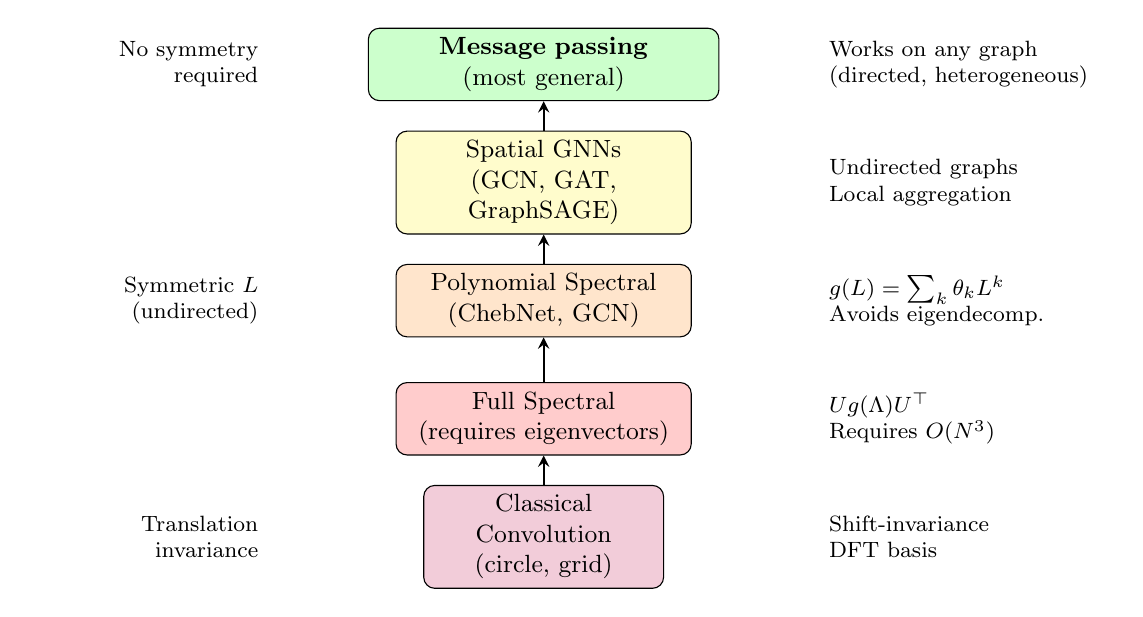
\begin{tikzpicture}[
    concept/.style={rectangle, draw, rounded corners, fill=blue!10,
                    text width=7em, minimum height=2.5em,
                    text centered, font=\small},
    arrow/.style={->, >=stealth, thick}
]

% Hierarchy
\node[concept, fill=green!20, text width=12em] (mp) at (0, 3)
    {\textbf{Message passing}\\(most general)};

\node[concept, fill=yellow!20, text width=10em] (spatial) at (0, 1.5)
    {Spatial GNNs\\(GCN, GAT, GraphSAGE)};

\node[concept, fill=orange!20, text width=10em] (poly) at (0, 0)
    {Polynomial Spectral\\(ChebNet, GCN)};

\node[concept, fill=red!20, text width=10em] (spectral) at (0, -1.5)
    {Full Spectral\\(requires eigenvectors)};

\node[concept, fill=purple!20, text width=8em] (classical) at (0, -3)
    {Classical Convolution\\(circle, grid)};

% Arrows showing "special case of"
\draw[arrow] (spatial) -- (mp);
\draw[arrow] (poly) -- (spatial);
\draw[arrow] (spectral) -- (poly);
\draw[arrow] (classical) -- (spectral);

% Annotations
\node[right, font=\footnotesize, text width=10em] at (3.5, 3)
    {Works on any graph\\(directed, heterogeneous)};
\node[right, font=\footnotesize, text width=10em] at (3.5, 1.5)
    {Undirected graphs\\Local aggregation};
\node[right, font=\footnotesize, text width=10em] at (3.5, 0)
    {$g(L) = \sum_k \theta_k L^k$\\Avoids eigendecomp.};
\node[right, font=\footnotesize, text width=10em] at (3.5, -1.5)
    {$U g(\Lambda) U^\top$\\Requires $O(N^3)$};
\node[right, font=\footnotesize, text width=10em] at (3.5, -3)
    {Shift-invariance\\DFT basis};

% Left annotations - requirements
\node[left, font=\footnotesize, text width=8em, align=right] at (-3.5, 3)
    {No symmetry\\required};
\node[left, font=\footnotesize, text width=8em, align=right] at (-3.5, 0)
    {Symmetric $L$\\(undirected)};
\node[left, font=\footnotesize, text width=8em, align=right] at (-3.5, -3)
    {Translation\\invariance};

\end{tikzpicture}
\caption{The hierarchy of graph neural network methods. Each level is
         a special case of the one above: on a fixed graph every spectral filter is a polynomial in $L$ (of degree below the number of distinct eigenvalues), and classical circular convolution is a spectral filter when its kernel is symmetric. Message passing is the most
         general framework.}
\label{dft-to-gnn:fig:hierarchy}
\end{figure}

\subsection{When to use which approach}

\begin{itemize}
    \item \textbf{Full spectral methods}: Rarely used in practice due
          to $O(N^3)$ cost. Useful for theoretical analysis and small
          graphs.

    \item \textbf{Polynomial spectral (ChebNet, GCN)}: Good balance of
          theory and practice. The spectral interpretation helps
          understand what the network learns (low-pass vs.\ high-pass
          filters).

    \item \textbf{General message passing (GAT, GraphSAGE)}: Most
          flexible. Use when you have directed graphs, edge features,
          heterogeneous node types, or need inductive learning (applying
          to new graphs).
\end{itemize}

\begin{remark}[The value of the spectral perspective]
Even though message passing is more general and practical, the spectral
perspective remains valuable:

\begin{enumerate}
    \item It explains \emph{why} GNNs work as frequency filters.
    \item It helps understand \emph{over-smoothing}: too many layers
          $\approx$ low-pass filter that kills all signal.
    \item It provides design principles: if you want to preserve
          high-frequency information, design filters accordingly.
    \item It connects to classical signal processing intuition.
\end{enumerate}

The spectral view is for \emph{understanding}; message passing is for
\emph{implementation}.
\end{remark}

%==========================================================================
\section{Key formulas}

\begin{center}
\renewcommand{\arraystretch}{1.6}
\begin{tabular}{ll}
\toprule
Concept & Formula \\
\midrule
DFT & $X_k = \sum_{n=0}^{N-1} x_n \, e^{-2\pi i kn/N}$ \\[0.3em]
Inverse DFT & $x_n = \frac{1}{N} \sum_{k=0}^{N-1} X_k \,
              e^{2\pi i kn/N}$ \\[0.3em]
Circular convolution & $y_n = \sum_{m=0}^{N-1} x_m h_{(n-m) \bmod N}$ \\[0.3em]
Circular conv.\ theorem & $\text{DFT}(\mathbf{x} \circledast \mathbf{h})
                         = \text{DFT}(\mathbf{x}) \odot
                           \text{DFT}(\mathbf{h})$ \\[0.3em]
Linear conv.\ via DFT & Zero-pad to $L \geq N+M-1$, then use circular \\[0.3em]
Graph Laplacian & $L = D - A$ \\[0.3em]
Graph Fourier transform & $\hat{\mathbf{x}} = U^\top \mathbf{x}$ where
                          $L = U\Lambda U^\top$ \\[0.3em]
Spectral graph conv.\ & $\mathbf{x} *_G g
                        = U \, g(\Lambda) \, U^\top \mathbf{x}$ \\[0.3em]
Message passing & $h_i^{(l+1)} = \phi\bigl( h_i^{(l)},
                  \bigoplus_{j \in \mathcal{N}(i)}
                  \psi(h_i^{(l)}, h_j^{(l)}, e_{ji}) \bigr)$ \\[0.3em]
GCN layer & $H^{(l+1)} = \sigma(\hat{D}^{-1/2}\hat{A}
            \hat{D}^{-1/2} H^{(l)} W^{(l)})$ \\
\bottomrule
\end{tabular}
\end{center}


\begin{chaptersummary}
\begin{itemize}
\item The Laplacian of the cycle $C_N$ is $L_N = 2I - A_N$; its eigenvectors are the DFT vectors $\mathbf{v}_k$ with eigenvalues $4\sin^2(\pi k/N)$, so the DFT is the expansion of a signal in the eigenbasis of $L_N$. Any matrix commuting with the cyclic shift has these eigenvectors.
\item Every circulant matrix $C$ satisfies $C = F^{-1}\diag(F\mathbf{c})F$; since circular convolution is multiplication by a circulant matrix, $\mathrm{DFT}(\mathbf{x}\circledast\mathbf{h}) = \mathrm{DFT}(\mathbf{x})\odot\mathrm{DFT}(\mathbf{h})$. Zero padding to length at least $N+M-1$ makes circular convolution equal linear convolution, which the FFT then computes in $O(L\log L)$.
\item On a general undirected graph, $L = U\Lambda U^\top$ defines the graph Fourier transform $\hat{\mathbf{x}} = U^\top\mathbf{x}$ and spectral filters $U g(\Lambda)U^\top$. This is a definition by analogy; on the cycle it recovers circular convolution with symmetric kernels.
\item Polynomial filters $g(L) = \sum_k\theta_kL^k$ need no eigenvectors and are local: a degree-$K$ polynomial only mixes nodes within distance $K$. ChebNet parametrizes them with Chebyshev polynomials of the rescaled Laplacian; GCN keeps degree one, ties the two coefficients and renormalizes, giving $H^{(l+1)} = \sigma(\hat D^{-1/2}\hat A\hat D^{-1/2}H^{(l)}W^{(l)})$.
\item Spectral methods need a symmetric $L$, cost $O(N^3)$ for the eigendecomposition, and are tied to one graph. For directed graphs $L$ can have complex eigenvalues or fail to be diagonalizable.
\item Message passing (message, aggregate, update) works on any graph at cost $O(\abs{E})$ per layer. GCN, GraphSAGE and GAT are instances, and every polynomial spectral filter of degree $K$ is $K$ rounds of message passing.
\end{itemize}
\end{chaptersummary}

\chapterappendix
\section{Why complex exponentials? Translation invariance}
\label{dft-to-gnn:app:translation-invariance}
%==========================================================================

This appendix provides a detailed proof of why complex exponentials
are the eigenfunctions of the circular graph Laplacian. The key insight
is that this is forced by \emph{translation invariance}.

\subsection{The fundamental question}

We showed in \cref{dft-to-gnn:thm:circular-eigenvectors} that the eigenvectors of the circular graph
Laplacian are complex exponentials $e^{2\pi i kn/N}$. But \emph{why}
are complex exponentials special? Why not some other basis?

\subsection{Translation invariance}

A system is \emph{translation-invariant} (or shift-invariant) if
shifting the input shifts the output by the same amount. For a discrete
system on the circle, define the shift operator:
\[
(T_a \mathbf{x})_n = x_{(n-a) \bmod N}
\]
A linear operator $L$ is translation invariant if it commutes with every shift:
\[
L T_a = T_a L \quad \text{for all } a .
\]

The circular graph Laplacian satisfies this property because every node
``looks the same'' as every other node --- the graph has perfect rotational
symmetry.

\subsection{The main theorem}

\begin{theorem}[Exponentials as forced eigenfunctions]
\label{dft-to-gnn:thm:app-forced-eigenfunctions}
Let $L$ be an $N\times N$ matrix that commutes with the cyclic shift, $LT_1 = T_1L$ (equivalently, with all $T_a$). Then each Fourier vector $\mathbf{v}_k = N^{-1/2}(e^{2\pi i kn/N})_{n=0}^{N-1}$, $k = 0, \ldots, N-1$, is an eigenvector of $L$. In particular $L$ is diagonalized by the DFT, and if an eigenvalue of $L$ is simple, its eigenvectors are multiples of a single $\mathbf{v}_k$.
\end{theorem}

\begin{proof}
\emph{Step 1: the eigenvectors of the shift.} Write $T = T_1$, so $(T\mathbf{x})_n = x_{(n-1)\bmod N}$ and $T_a = T^a$. Suppose $T\mathbf{v} = \mu\mathbf{v}$ with $\mathbf{v} \ne 0$. Componentwise, $v_{n-1} = \mu v_n$, so $v_n = \mu^{-n}v_0$ for all $n$, and $v_0 \ne 0$. Going once around the circle, $T^N = I$ gives $\mu^N = 1$, so $\mu = e^{-2\pi i k/N}$ for some $k\in\{0, \ldots, N-1\}$, and then $v_n = v_0\,e^{2\pi i kn/N}$: the eigenvectors of $T$ are exactly the multiples of the $\mathbf{v}_k$. The $N$ eigenvalues $e^{-2\pi i k/N}$ are distinct, so each eigenspace of $T$ is one-dimensional.

\emph{Step 2: commuting matrices preserve eigenspaces.} If $T\mathbf{v}_k = \mu_k\mathbf{v}_k$, then $T(L\mathbf{v}_k) = L(T\mathbf{v}_k) = \mu_k(L\mathbf{v}_k)$, so $L\mathbf{v}_k$ lies in the eigenspace of $T$ for $\mu_k$. That space is spanned by $\mathbf{v}_k$, hence $L\mathbf{v}_k = c_k\mathbf{v}_k$ for some scalar $c_k$.

\emph{Step 3: conclusion.} The $\mathbf{v}_k$ are orthonormal and $L\mathbf{v}_k = c_k\mathbf{v}_k$, so $L = Q\diag(c_0,\ldots,c_{N-1})Q^*$ with $Q = [\mathbf{v}_0|\cdots|\mathbf{v}_{N-1}] = F^*/\sqrt N$. If an eigenvalue $c$ is simple, it equals $c_k$ for exactly one $k$, and its eigenspace is spanned by $\mathbf{v}_k$.
\end{proof}

\begin{remark}
The argument does not say that \emph{every} eigenvector of $L$ is an exponential. For the cycle Laplacian, $c_k = c_{N-k}$, and $\cos(2\pi kn/N)$ is an eigenvector of $L_N$ without being an eigenvector of $T$. What the symmetry forces is a common eigenbasis: the exponentials are the only basis that diagonalizes every shift-invariant operator simultaneously, which is why one transform serves all of them. The same reasoning on $\Z$ or $\R$, with the eigenfunctions $e^{i\omega t}$ of continuous translations, gives the convolution theorem of \cref{ch:fourier-analysis}.
\end{remark}

\subsection{The universal principle}

This result explains why Fourier analysis appears throughout science:

\begin{keyidea}
\emph{Any system that is translation-invariant is diagonalized by
complex exponentials.}
\end{keyidea}

\paragraph{Examples.}
\begin{itemize}
\item \textbf{Time-invariant linear systems} (signal processing):
      Time translation invariance $\Rightarrow$ frequency domain analysis.
\item \textbf{Spatially homogeneous media} (wave propagation):
      Space translation invariance $\Rightarrow$ spatial Fourier transforms.
\item \textbf{Crystals with periodic structure} (solid-state physics):
      Lattice translation invariance $\Rightarrow$ Bloch's theorem.
\item \textbf{Stationary random processes} (probability):
      Time translation invariance $\Rightarrow$ spectral density.
\end{itemize}

\subsection{Implications for graphs}

For general graphs without translational symmetry:
\begin{itemize}
\item There is no family of shifts acting transitively on the nodes, unless the graph has that much symmetry (as the cycle or the torus grid does); the Laplacian commutes only with the permutations that are automorphisms of the graph.
\item Eigenvectors are \emph{not} complex exponentials.
\item But the eigenvectors still provide a natural ``frequency basis''
      (ordered by eigenvalue = smoothness).
\end{itemize}

This is why spectral graph convolution \emph{defines} frequency analysis
using Laplacian eigenvectors, rather than \emph{deriving} it from
symmetry principles. The circular graph is special precisely because
it has the translation symmetry that forces the exponential basis.

%==========================================================================
\section{The path graph and the discrete cosine transform}
\label{dft-to-gnn:app:dct-path}
%==========================================================================

Just as the circular graph leads to the DFT, the \emph{path graph}
leads to the \emph{Discrete Cosine Transform (DCT)}. This appendix
proves this connection and explains why boundary conditions matter.

\subsection{The path graph Laplacian}

The path graph $P_N$ has $N$ nodes connected in a line:
\begin{center}
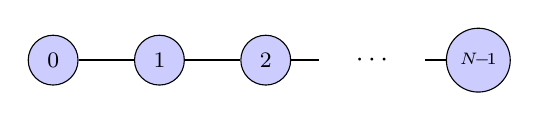
\begin{tikzpicture}[scale=0.9]
    \foreach \i in {0,1,2} {
        \node[circle, draw, fill=blue!20, minimum size=18pt]
            (n\i) at (\i*1.5, 0) {\footnotesize $\i$};
    }
    \node at (4.5, 0) {$\cdots$};
    \node[circle, draw, fill=blue!20, minimum size=18pt]
        (nm1) at (6, 0) {\footnotesize $\scriptstyle N\!-\!1$};

    \draw[thick] (n0) -- (n1) -- (n2) -- (3.75, 0);
    \draw[thick] (5.25, 0) -- (nm1);
\end{tikzpicture}
\end{center}

Unlike the circular graph, there is \emph{no edge} from node $N-1$
back to node $0$. The Laplacian is:
\[
L_{\text{path}} = \begin{pmatrix}
1 & -1 & 0 & \cdots & 0 \\
-1 & 2 & -1 & \cdots & 0 \\
0 & -1 & 2 & \cdots & 0 \\
\vdots & & \ddots & \ddots & -1 \\
0 & 0 & \cdots & -1 & 1
\end{pmatrix}
\]

Note the \emph{boundary conditions}: the corner entries are $1$ (not
$2$) because the endpoints have degree $1$.

\subsection{Finding the eigenvectors}

For the interior nodes ($1 \leq n \leq N-2$), the eigenvalue equation
$L\mathbf{u} = \lambda \mathbf{u}$ gives:
\[
-u_{n-1} + 2u_n - u_{n+1} = \lambda u_n
\]

This is the same recurrence as for the circular graph. So we try
$u_n = e^{i\omega n}$, which gives:
\[
-e^{-i\omega} + 2 - e^{i\omega} = \lambda
\quad \Rightarrow \quad
\lambda = 2 - 2\cos\omega = 4\sin^2(\omega/2)
\]

The general solution is $u_n = A e^{i\omega n} + B e^{-i\omega n}$, or
equivalently:
\[
u_n = C \cos(\omega n) + D \sin(\omega n)
\]

\subsection{Applying boundary conditions}

Now we apply the boundary conditions. At $n = 0$:
\[
u_0 - u_1 = \lambda u_0 \quad \Rightarrow \quad
u_1 = (1 - \lambda) u_0
\]

At $n = N-1$:
\[
-u_{N-2} + u_{N-1} = \lambda u_{N-1} \quad \Rightarrow \quad
u_{N-2} = (1 - \lambda) u_{N-1}
\]

These are \emph{Neumann-like} boundary conditions (the discrete
analogue of $\frac{du}{dx} = 0$ at the boundary).

A convenient way to impose them is the \emph{ghost-node} trick. Extend $\mathbf u$ by $u_{-1} = u_0$ and $u_N = u_{N-1}$. Then the interior equation $-u_{n-1} + 2u_n - u_{n+1} = \lambda u_n$ at $n = 0$ reads $-u_0 + 2u_0 - u_1 = \lambda u_0$, which is the first boundary equation, and likewise at $n = N-1$. So we need a solution of the interior recurrence on $n = -1, \ldots, N$ with $u_{-1} = u_0$ and $u_N = u_{N-1}$.

The condition $u_{-1} = u_0$ says that $\mathbf u$ is symmetric about $n = -\frac12$, which suggests the ansatz $u_n = \cos\bigl(\omega(n+\frac12)\bigr)$. Indeed, $u_{-1} = \cos(-\omega/2) = \cos(\omega/2) = u_0$. At the other end, using $\cos a - \cos b = -2\sin\frac{a+b}{2}\sin\frac{a-b}{2}$,
\[
u_N - u_{N-1} = \cos\bigl(\omega(N+\tfrac12)\bigr) - \cos\bigl(\omega(N-\tfrac12)\bigr) = -2\sin(\omega N)\sin(\omega/2),
\]
which vanishes when $\omega N = k\pi$. The values $k = 0, 1, \ldots, N-1$ give $\omega \in [0, \pi)$ and $N$ distinct eigenvalues $2 - 2\cos(\pi k/N)$, hence a complete set of eigenvectors (other integers $k$ repeat these, up to sign, or give $u = 0$).

\subsection{The DCT-II basis}

Combining these results, the eigenvectors of the path graph are:

\begin{theorem}[Path graph eigenvectors = DCT-II basis]
\label{dft-to-gnn:thm:path-dct}
The eigenvectors of the path graph Laplacian $L_{P_N}$ are:
\begin{equation}
u_k[n] = \sqrt{\frac{2 - \delta_{k0}}{N}} \cos\left(\frac{\pi k (n + \frac{1}{2})}{N}\right),
\quad k = 0, 1, \ldots, N-1
\end{equation}
with eigenvalues:
\begin{equation}
\lambda_k = 4\sin^2\left(\frac{\pi k}{2N}\right) =
2\left(1 - \cos\frac{\pi k}{N}\right)
\end{equation}
where $\delta_{k0}$ is the Kronecker delta (the normalization factor
is $\sqrt{1/N}$ for $k=0$ and $\sqrt{2/N}$ for $k > 0$).
\end{theorem}

These are exactly the basis vectors of the \emph{DCT-II} (the most
common DCT variant, often just called ``the DCT'').

\subsection{Comparison: DFT vs.\ DCT}

\begin{center}
\renewcommand{\arraystretch}{1.4}
\begin{tabular}{lcc}
\toprule
Property & DFT (circular graph) & DCT (path graph) \\
\midrule
Graph structure & Circle (periodic) & Path (endpoints) \\
Boundary condition & Periodic: $u_{N} = u_0$ & Neumann-like \\
Basis functions & $e^{2\pi i kn/N}$ & $\cos\left(\frac{\pi k(n+1/2)}{N}\right)$ \\
Eigenvalues & $4\sin^2(\pi k/N)$ & $4\sin^2(\pi k/2N)$ \\
Values & Complex & Real \\
Symmetry & Translation invariance & Reflection symmetry \\
\bottomrule
\end{tabular}
\end{center}

\subsection{Why this matters}

\begin{enumerate}
\item \textbf{Boundary conditions determine the transform.} The same
      differential operator (second derivative / graph Laplacian) gives
      different eigenvectors depending on boundary conditions:
      \begin{itemize}
          \item Periodic boundaries $\rightarrow$ DFT (complex exponentials).
          \item Neumann boundaries $\rightarrow$ DCT (cosines).
          \item Dirichlet boundaries ($u = 0$ at endpoints) $\rightarrow$
                DST (Discrete Sine Transform).
      \end{itemize}

\item \textbf{The DCT is widely used in practice.} JPEG image compression
      uses the DCT precisely because images have boundaries (edges) rather
      than periodic structure. The DCT handles boundaries more naturally
      than the DFT.

\item \textbf{General graphs have no such structure.} For an arbitrary
      graph, there is no clean formula for the eigenvectors --- they must
      be computed numerically. The path and circle are special because
      their regularity allows closed-form solutions.
\end{enumerate}

\begin{figure}[H]
\centering
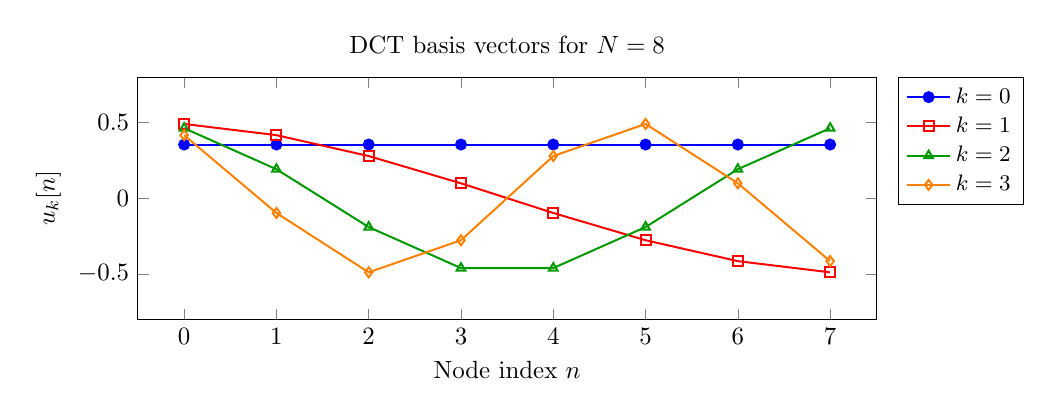
\begin{tikzpicture}[scale=0.9]
\begin{axis}[
    width=12cm, height=5cm,
    xlabel={Node index $n$},
    ylabel={$u_k[n]$},
    xmin=-0.5, xmax=7.5,
    ymin=-0.8, ymax=0.8,
    legend pos=outer north east,
    legend style={font=\small},
    title={DCT basis vectors for $N=8$}
]
% k=0 (constant)
\addplot[thick, blue, mark=*] coordinates {
    (0,0.354) (1,0.354) (2,0.354) (3,0.354)
    (4,0.354) (5,0.354) (6,0.354) (7,0.354)
};
\addlegendentry{$k=0$}

% k=1
\addplot[thick, red, mark=square, mark size=2pt] coordinates {
    (0,0.490) (1,0.416) (2,0.278) (3,0.098)
    (4,-0.098) (5,-0.278) (6,-0.416) (7,-0.490)
};
\addlegendentry{$k=1$}

% k=2
\addplot[thick, green!60!black, mark=triangle, mark size=2pt] coordinates {
    (0,0.462) (1,0.191) (2,-0.191) (3,-0.462)
    (4,-0.462) (5,-0.191) (6,0.191) (7,0.462)
};
\addlegendentry{$k=2$}

% k=3
\addplot[thick, orange, mark=diamond, mark size=2pt] coordinates {
    (0,0.416) (1,-0.098) (2,-0.490) (3,-0.278)
    (4,0.278) (5,0.490) (6,0.098) (7,-0.416)
};
\addlegendentry{$k=3$}
\end{axis}
\end{tikzpicture}
\caption{The first four DCT basis vectors for $N=8$. Compare with
         the cycle eigenvectors of \cref{dft-to-gnn:fig:cycle-eigvecs}: same qualitative behaviour (increasing oscillation
         with $k$) but adapted to path boundary conditions.}
\end{figure}

%==========================================================================
\section{Efficient matrix implementation for GPUs}
\label{dft-to-gnn:app:matrix-implementation}
%==========================================================================

The per-node message passing formulas are conceptually clear but
computationally inefficient. For GPU acceleration, we must express
everything as matrix operations. This appendix shows how.

\subsection{The challenge}

Consider the GCN update for node $i$:
\[
h_i^{(l+1)} = \sigma\left( \sum_{j \in \mathcal{N}(i) \cup \{i\}}
    \frac{1}{\sqrt{\hat{d}_i}\sqrt{\hat{d}_j}} h_j^{(l)} W^{(l)} \right)
\]

A naive implementation would loop over nodes and neighbours:
\begin{lstlisting}[language=Python]
for i in range(N):
    h_new[i] = 0
    for j in neighbors[i] + [i]:
        h_new[i] += h[j] @ W / sqrt(d_hat[i] * d_hat[j])
    h_new[i] = relu(h_new[i])
\end{lstlisting}

This performs $O(N\bar d)$ small vector-matrix products one after another, where $\bar d$ is the average degree; GPUs are fast at a few large matrix operations, not at many small sequential ones.

\subsection{Matrix form of GCN}

The key insight is that the normalized adjacency matrix
$\hat{P} = \hat{D}^{-1/2} \hat{A} \hat{D}^{-1/2}$ encodes all the
neighbourhood structure and normalization:
\[
\hat{P}_{ij} = \begin{cases}
\frac{1}{\sqrt{\hat{d}_i}\sqrt{\hat{d}_j}} & \text{if } j \in \mathcal{N}(i) \cup \{i\} \\
0 & \text{otherwise}
\end{cases}
\]

Then the entire GCN layer becomes:
\[
H^{(l+1)} = \sigma\left( \hat{P} \, H^{(l)} \, W^{(l)} \right)
\]

In code (PyTorch-style):
\begin{lstlisting}[language=Python]
H_new = relu(P_hat @ H @ W)
\end{lstlisting}

This is just two matrix multiplications and an elementwise nonlinearity --- highly
optimized on GPUs.

\subsection{Sparse matrix operations}

For large graphs, $\hat{P}$ is sparse (most entries are zero). We store
it in sparse format and use sparse-dense matrix multiplication:

\begin{lstlisting}[language=Python]
# P_hat is sparse (N x N), H is dense (N x d), W is dense (d x d')
H_new = relu(sparse_mm(P_hat, H) @ W)
\end{lstlisting}

Complexity: $O(|E| \cdot d + N \cdot d \cdot d')$ instead of $O(N^2 \cdot d)$.

\subsection{Matrix form of GAT}

GAT is trickier because attention weights depend on node features. The
key steps are:

\paragraph{Step 1: compute all transformed features.}
\[
Z = H W \in \mathbb{R}^{N \times d'}
\]
where row $z_i = h_i W \in \mathbb{R}^{1 \times d'}$ is the transformed
feature vector for node $i$.

\paragraph{Step 2: compute attention scores for all edges.}

For each edge $(i,j)$, we need to compute an attention score. Following
the GAT formula, this involves:
\begin{itemize}
    \item $[z_i \| z_j]$: concatenation of the two row vectors, giving
          a row vector in $\mathbb{R}^{1 \times 2d'}$.
    \item $\mathbf{a} \in \mathbb{R}^{2d'}$: a learnable column vector.
    \item $[z_i \| z_j] \, \mathbf{a}$: the dot product, giving a scalar.
\end{itemize}

\paragraph{The decomposition trick.} Naively computing $[z_i \| z_j]$ for
all $|E|$ edges is expensive. Instead, we split $\mathbf{a}$ into two
halves:
\[
\mathbf{a} = \begin{pmatrix} \mathbf{a}_1 \\ \mathbf{a}_2 \end{pmatrix}
\quad \text{where } \mathbf{a}_1, \mathbf{a}_2 \in \mathbb{R}^{d'}
\]

Then:
\[
[z_i \| z_j] \mathbf{a} = [z_i \| z_j] \begin{pmatrix} \mathbf{a}_1 \\ \mathbf{a}_2 \end{pmatrix}
= z_i \mathbf{a}_1 + z_j \mathbf{a}_2
\]

So we can precompute two vectors of size $N$ (one per node):
\begin{align*}
\mathbf{s}_1 &= Z \mathbf{a}_1 \in \mathbb{R}^{N} \quad \text{(score contribution from source node)} \\
\mathbf{s}_2 &= Z \mathbf{a}_2 \in \mathbb{R}^{N} \quad \text{(score contribution from target node)}
\end{align*}

The attention score for edge $(i,j)$ is then simply:
\[
e_{ij} = \text{LeakyReLU}(s_{1,i} + s_{2,j})
\]

This avoids forming $|E|$ concatenated vectors --- we just index into two
precomputed vectors of size $N$.

\paragraph{Step 3: evaluate the scores on the edge list.}
We compute $e_{ij}$ only for pairs in which $j$ sends to $i$, that is $j \in \mathcal N(i)\cup\{i\}$ (the self-loops are added to the edge list). In $e_{ij}$ the receiving node $i$ uses $\mathbf a_1$ and the sender $j$ uses $\mathbf a_2$:
\begin{lstlisting}[language=Python]
# edge_index: (2, |E|) tensor; edge_index[0] = senders j, edge_index[1] = receivers i
src, dst = edge_index
e = leaky_relu(s1[dst] + s2[src])  # e_ij for each edge j -> i, shape (|E|,)
\end{lstlisting}

\paragraph{Step 4: softmax per node.}

Apply softmax over each node's incoming edges (all edges with the same
target node):
\begin{lstlisting}[language=Python]
# For each receiver i, softmax over its incoming edges
alpha = sparse_softmax(e, index=dst, num_nodes=N)
\end{lstlisting}

\paragraph{Step 5: aggregate.}

Construct a sparse attention matrix $A_{\text{att}}$ with $(A_{\text{att}})_{ij} = \alpha_{ij}$ when $j$ sends to $i$ and $0$ otherwise (row $i$ = receiver), so that row $i$ of $A_{\text{att}}Z$ is $\sum_j\alpha_{ij}z_j$. The final aggregation is:
\begin{lstlisting}[language=Python]
# A_att: (N, N) sparse matrix with attention weights
H_new = sparse_mm(A_att, Z)  # shape: (N, d')
\end{lstlisting}

\subsection{General message passing in matrix form}

For a general message passing layer:
\[
h_i^{(l+1)} = \phi\left( h_i^{(l)}, \bigoplus_{j \in \mathcal{N}(i)}
    \psi(h_i^{(l)}, h_j^{(l)}, e_{ij}) \right)
\]

The matrix implementation depends on the specific $\psi$ and $\bigoplus$:

\begin{center}
\renewcommand{\arraystretch}{1.3}
\begin{tabular}{lll}
\toprule
Aggregation $\bigoplus$ & Matrix operation & Notes \\
\midrule
Sum & $A \cdot H$ & Sparse matrix multiply \\
Mean & $D^{-1} A \cdot H$ & Row-normalized \\
Max & \texttt{scatter\_max} & Requires scatter ops \\
Attention & $\text{Softmax}(E) \cdot H$ & Row-wise softmax over neighbours only \\
\bottomrule
\end{tabular}
\end{center}

\subsection{Example: complete GCN forward pass}

\begin{example}[GCN in PyTorch]
Here is a complete GCN layer implementation:

\begin{lstlisting}[language=Python]
import torch
import torch.nn as nn

class GCNLayer(nn.Module):
    def __init__(self, in_dim, out_dim):
        super().__init__()
        self.W = nn.Parameter(torch.randn(in_dim, out_dim))

    def forward(self, H, P_hat):
        """
        H: (N, in_dim) node features
        P_hat: (N, N) sparse normalized adjacency
        """
        # Aggregate then transform
        H_agg = torch.sparse.mm(P_hat, H)  # (N, in_dim)
        H_new = H_agg @ self.W              # (N, out_dim)
        return torch.relu(H_new)
\end{lstlisting}

The preprocessing (computing $\hat{P}$ from $A$) is done once:
\begin{lstlisting}[language=Python]
def compute_P_hat(A, N):
    """A: (N, N) dense adjacency matrix (convert to sparse at the end)"""
    A_hat = A + torch.eye(N)           # Add self-loops
    D_hat = A_hat.sum(dim=1)           # Degrees
    D_inv_sqrt = D_hat.pow(-0.5)
    # P_hat = D^{-1/2} A_hat D^{-1/2}
    P_hat = D_inv_sqrt.view(-1,1) * A_hat * D_inv_sqrt.view(1,-1)
    return P_hat.to_sparse()
\end{lstlisting}
\end{example}

\subsection{Batching multiple graphs}

For batching multiple graphs (common in graph classification), we
create a block-diagonal adjacency matrix:

\[
A_{\text{batch}} = \begin{pmatrix}
A_1 & 0 & 0 \\
0 & A_2 & 0 \\
0 & 0 & A_3
\end{pmatrix}, \quad
H_{\text{batch}} = \begin{pmatrix}
H_1 \\ H_2 \\ H_3
\end{pmatrix}
\]

The same matrix operations work on the batched data, with no
cross-graph message passing (ensured by the block structure).

%==========================================================================
\section*{Further reading}
\addcontentsline{toc}{section}{Further reading}
Shuman et al.\ (\emph{The Emerging Field of Signal Processing on Graphs}, 2013) survey graph Fourier transforms and filters; Chung (\emph{Spectral Graph Theory}, 1997) is the classical reference for Laplacian spectra, and Strang (\emph{The Discrete Cosine Transform}, 1999) explains the DCT through boundary conditions, as in the appendix. Spectral graph networks start with Bruna et al.\ (\emph{Spectral Networks and Locally Connected Networks on Graphs}, 2014); ChebNet is due to Defferrard, Bresson and Vandergheynst (2016) and GCN to Kipf and Welling (2017). Message passing was formulated by Gilmer et al.\ (2017); GraphSAGE and GAT are by Hamilton, Ying and Leskovec (2017) and Veličković et al.\ (2018). Bronstein et al.\ (\emph{Geometric Deep Learning}, 2021) place all of these in a framework of symmetries, and Wu et al.\ (\emph{A Comprehensive Survey on Graph Neural Networks}, 2020) is a broad survey. Calder and Olver (\emph{Linear Algebra, Data Science, and Machine Learning}, 2025) treat graph Laplacians and their spectra at textbook level.


\section*{Exercises}
\addcontentsline{toc}{section}{Exercises}

\begin{exercise}\label{dft-to-gnn:exr:1}
Show that the cycle Laplacian $L_N$ is a circulant matrix with first column $\mathbf c = (2, -1, 0, \ldots, 0, -1)^\top$, and use \cref{dft-to-gnn:thm:circulant-eigenvectors} to rederive its eigenvalues $\lambda_k = 2 - 2\cos(2\pi k/N)$. List them for $N = 4$.
\solutionlink{dft-to-gnn:exr:1}
\end{exercise}

\begin{exercise}\label{dft-to-gnn:exr:2}
On the path $0 - 1 - 2$, the Laplacian has eigenvalues $0, 1, 3$. Find the polynomial $p(\lambda) = 1 + a\lambda + b\lambda^2$ with $p(\lambda_k) = e^{-\lambda_k}$ for the three eigenvalues, so that the heat kernel $e^{-L}$ equals $p(L)$. Use \cref{dft-to-gnn:lem:local} to explain why $(e^{-L})_{20} = b$, and give its value.
\hint{$(L^2)_{20} = L_{21}L_{10}$.}
\solutionlink{dft-to-gnn:exr:2}
\end{exercise}

\begin{exercise}\label{dft-to-gnn:exr:3}
Let $x = (1, -1)$ and $h = (1, 2, 1)$. Compute the linear convolution $x * h$, and the circular convolution of length $3$ of $(1, -1, 0)$ with $h$. Show that the second is obtained from the first by folding entry $3$ onto entry $0$, and give the smallest length for which the DFT method returns $x*h$.
\solutionlink{dft-to-gnn:exr:3}
\end{exercise}

\begin{exercise}\label{dft-to-gnn:exr:4}
Let $\hat A = A + I$, $\hat D = D + I$ and $\hat P = \hat D^{-1/2}\hat A\hat D^{-1/2}$ for an undirected graph with maximal degree $d_{\max}$. Show that every eigenvalue $\mu$ of $\hat P$ satisfies $-1 + \frac{2}{d_{\max}+1} \le \mu \le 1$. Show that without self-loops, $D^{-1/2}AD^{-1/2}$ has eigenvalue $-1$ on a bipartite graph.
\hint{Write $I \mp \hat P$ as $\hat D^{-1/2}(\hat D \mp \hat A)\hat D^{-1/2}$ and use $\mathbf x^\top(D + A)\mathbf x = \sum_{(i,j)\in E}A_{ij}(x_i + x_j)^2$.}
\solutionlink{dft-to-gnn:exr:4}
\end{exercise}

\begin{exercise}\label{dft-to-gnn:exr:5}
Let $f(A, H) = \sigma(\hat D^{-1/2}\hat A\hat D^{-1/2}HW)$ be a GCN layer and $\Pi$ a permutation matrix (a relabelling of the nodes). Show that $f(\Pi A\Pi^\top, \Pi H) = \Pi f(A, H)$: the layer is \emph{permutation equivariant}. Why is this the right property for a function of a graph whose node numbering is arbitrary?
\solutionlink{dft-to-gnn:exr:5}
\end{exercise}
\end{notechapter}
